% !TeX spellcheck = en_US
\documentclass[preprint,authoryear]{elsarticle}
% sudo apt-get install -y texlive-publishers

\usepackage[left]{lineno}
\usepackage[utf8]{inputenc}
\usepackage[T1]{fontenc}
\usepackage{lmodern}
\usepackage{multirow}

\usepackage{lineno,hyperref}
\modulolinenumbers[5]

\usepackage[none]{hyphenat}

\usepackage{url}
\usepackage{booktabs}

\usepackage{mathtools}
\usepackage{amssymb}
\usepackage{amsthm}
%\usepackage{amsmath}

\usepackage{caption}
\captionsetup{labelfont=bf}
\captionsetup{skip=0pt} % vertical distance from the table or figure


\usepackage{algorithm} % sudo apt-get install -y texlive-science

\usepackage[noend]{algpseudocode}

\usepackage[margin=0.9in]{geometry}

\usepackage[normalem]{ulem}
\usepackage{xcolor}

\newcommand{\Comentar}[1]{\State {\cmmt{#1}}}
\newcommand{\Break}{\State \bf {break}}
\renewcommand{\Return}{\State \bf {return}~}
\renewcommand{\algorithmicensure}{\bf {Parameters:}}

\renewcommand\algorithmicthen{}
\renewcommand\algorithmicdo{}


\algblock{ForEach}{EndFor}
\algblock{ForDownTo}{EndFor}
\algblock{ForTo}{EndFor}

\newcommand{\Block}[1]{\State #1 \{}
\newcommand{\EndBlock}{\State \}}

%----- begin celio
\usepackage{scrextend}
\newcommand{\boldm}[1] {\mathversion{bold}#1\mathversion{normal}}
\newcommand{\round}[1]{\ensuremath{\lfloor#1\rceil}}
\usepackage{setspace}
\usepackage{array}
\usepackage{color, colortbl}
\definecolor{Gray}{gray}{0.9}

\newcommand{\specialcell}[2][c]{%
	\begin{tabular}[#1]{@{}c@{}}#2\end{tabular}}

\usepackage{tikz}
\usetikzlibrary{calc}
\usetikzlibrary{positioning}

\usepackage{pgfplots}

\pgfplotsset{
	compat=1.9,
	myplotstyle/.style={
		legend cell align=left,
		every axis plot/.append style={thick},
		legend style={font=\small,draw=none},
		enlargelimits=0.2,
		legend pos=south east,
		y tick label style={ /pgf/number format/.cd, fixed, fixed zerofill, precision=3, /tikz/.cd, },
		x tick label style={ /pgf/number format/.cd, fixed, fixed zerofill, precision=1, /tikz/.cd, },
		grid=major,		
	},
}

\usepackage{float}% http://ctan.org/pkg/float


%----- end celio

\journal{Computers \& Operations Research}


\begin{document}


\begin{frontmatter}

\title{Parallel air palletization and tour planning for simultaneous pickup and delivery}

\author{A.C.P.~Mesquita}
\ead{celio@ita.br}

\author{C.A.A.~Sanches\corref{cor1}}
\ead{alonso@ita.br}
\cortext[cor1]{Corresponding author.}

\address {Instituto Tecnol\'{o}gico de Aeron\'{a}utica - DCTA/ITA/IEC\\
Pra\c{c}a Mal. Eduardo Gomes, 50\\
S\~{a}o Jos\'{e} dos Campos - SP - 12.228-900 - Brazil}


\begin{abstract}

Parallelism is crucial for mobile computers to be capable of doing complicated operations while conserving energy. By leveraging parallelism, handheld computers can divide tasks into numerous smaller sections and execute these parts simultaneously, so utilizing multiple cores of the processor and offering a substantial performance improvement. This enables for more complicated applications and speedier performance, making mobile computers more competent than ever before.

In this work, we explore computer parallelism in solving the problem involving scheduling the loading and routing of an airplane in a tour of simultaneous pickup and delivery at intermediate hubs while taking into account a utility score, weight and balance rules, and fuel usage.

This hard problem, named {\it Air Cargo Load Planning with Routing, Pickup, and Delivery Problem} considers using standardized pallets in fixed positions, obeying the center of gravity constraints, delivering each item to its destination, and minimizing fuel consumption costs.

We also contributed by carrying out multiple experiments with the {\it Shims} heuristic on synthetic data based on real data from the {\it Brazilian Air Force} transportation history and a new procedure to minimize the distance from the next node destined pallet to the ramp door.

We converted {\it Shims} into a process-based parallel computing heuristic that quickly finds good solutions for a wide range of problem sizes, an essential contribution as it surpassed all {\it Shims} results.

\end{abstract}

\begin{keyword}
Air Cargo \sep Air Palletization \sep Weight and Balance \sep Pickup and Delivery \sep Parallel computing \sep iRace
\end{keyword}

\end{frontmatter}

\label{sec1}
\section{Introduction}


Air cargo transport involves several sub-problems that are difficult to solve. Recently, \cite{MesquitaSanches2023} modeled and solved the {\it Air Cargo Load Planning with Routing, Pickup and Delivery} (ACLP+RPDP) composed by four sub-problems: {\it Build-up Scheduling Problem}, {\it Air Palletization Problem} (APP), {\it Weight and Balance Problem} (WBP), and a special case of the {\it Traveling Salesman Problem}, similar to the proposed by \cite{kaspi2019}, where the profit per unit time is defined as the profit gained after completing the tour divided by the total time (cost in our case) required to complete the tour.

However, there are still other important challenges in air cargo transport that go beyond the definition of the ACLP+RPDP, especially with regard to algorithms performance and the easiness of loading operations at each destination.

Considering air cargo transport, Table \ref{tab:sa} lists the main works in the literature and the corresponding sub-problems addressed. We also indicate whether the dimensions of the items were taken into account ({\bf 3D} or {\bf 2D}) and which solution method was used: heuristics ({\bf Heu}), integers ({\bf Int}), or linear programming ({\bf Lin}).

\begin{table}[H]
	\centering
	\caption{Air cargo transport: literature, problems and features}  \label{tab:sa}
	\scriptsize
	\renewcommand{\arraystretch}{1.1} % alturas das linhas \specialcell{{\bf Parallel}\\{\bf heuristics}}
	\begin{tabular}{r|ccc|cc|cc|ccc|c}
		\toprule
		                            & {\bf APP}  & {\bf WBP}   & {\bf MLU} &{\bf SPDP}&{\bf TSP} & {\bf 2D} & {\bf 3D} & {\bf Heu} & {\bf Int}  & {\bf Lin} & \specialcell{{\bf Parallel}\\{\bf heuristics}}\\
		\midrule
		\cite{LarsenMikkelsen1979}  & $.$        & $\bigstar$  & $.$       & $.$      & $.$      & $.$      & $.$      & $\bigstar$& $.$        &  $.$       &  $.$ \\
		\cite{Brosh1981}            & $.$        & $\bigstar$  & $.$       & $.$      & $.$      & $.$      & $.$      & $.$       & $.$        &  $\bigstar$&  $.$ \\
		\cite{Kevin1992}            & $.$        & $\bigstar$  & $.$       & $.$      & $.$      & $.$      & $.$      & $.$       & $\bigstar$ &  $.$       &  $.$\\
		\cite{Heidelberg1998}       & $.$        & $\bigstar$  & $.$       & $.$      & $.$      &$\bigstar$& $.$      & $\bigstar$& $.$        &  $.$       &  $.$ \\
		\cite{MongeauBes2003}       & $\bigstar$ & $\bigstar$  & $.$       & $.$      & $.$      & $.$      & $.$      & $.$       & $\bigstar$ &  $.$       &  $.$\\
		\cite{fok2004optimizing}    & $.$        & $\bigstar$  & $.$       & $.$      & $.$      & $.$      & $.$      & $.$       & $\bigstar$ &  $.$       &  $.$ \\	
		\cite{Chan2006}             & $\bigstar$ & $.$         & $.$       & $.$      & $.$      & $.$      &$\bigstar$& $\bigstar$& $.$        &  $.$       &  $.$ \\
		\cite{KaluznyBohdanL2009Oalb}& $.$       & $\bigstar$  & $.$       & $.$      & $.$      &$\bigstar$& $.$      & $.$       & $\bigstar$ &  $.$       &  $.$ \\
		\cite{Verstichel2011}       & $.$        & $\bigstar$  & $.$       & $.$      & $.$      & $.$      & $.$      & $.$       & $\bigstar$ &  $.$       &  $.$ \\
		\cite{MesquitaCunha2011}    & $.$        & $.$         & $.$       &$\bigstar$& $.$      & $.$      & $.$      & $\bigstar$& $.$        &  $.$       &  $.$ \\		
		\cite{Limbourg2012}         & $.$        & $\bigstar$  & $.$       & $.$      & $.$      & $.$      & $.$      & $.$       & $\bigstar$ &  $.$       &  $.$ \\
		
		\cite{kaspi2019}            & $.$        & $.$         & $.$       & $.$      &$\bigstar$& $.$      & $.$      &$\bigstar$ & $.$        &  $.$       &  $.$ \\
		
		\cite{RoesenerHall2014}     & $\bigstar$ & $\bigstar$  & $.$       & $.$      & $.$      & $.$      &$\bigstar$& $.$       & $\bigstar$ &  $.$       &  $.$ \\
		\cite{Vancroonemburg2014}   & $\bigstar$ & $\bigstar$  & $.$       & $.$      & $.$      & $.$      & $.$      & $.$       & $\bigstar$ &  $.$       &  $.$ \\
		\cite{LurkinSchyns2015}     & $.$        & $\bigstar$  & $\bigstar$&$\bigstar$& $.$      & $.$      & $.$      & $.$       & $\bigstar$ &  $.$       &  $.$ \\
		\cite{RoesenerBarnes2016}   & $.$        & $\bigstar$  & $.$       & $.$      & $.$      & $.$      & $.$      & $\bigstar$& $.$        &  $.$       &  $.$ \\
		
		\cite{PaquaySchynsLimbourg2016,PaquayLimbourgSchynsOliveira2018}&$\bigstar$&$.$&$.$&$.$&$.$&$.$     &$\bigstar$&$\bigstar$ & $\bigstar$&$\bigstar$  &  $.$ \\
		
		\cite{YangLiuGao2018}       & $.$        & $\bigstar$  & $.$       & $.$      & $.$      &$\bigstar$& $.$      & $\bigstar$ & $.$       & $.$        &  $.$ \\
		\cite{wong2020}             & $\bigstar$ & $\bigstar$  & $.$       & $.$      & $.$      & $.$      & $.$      & $.$        & $\bigstar$& $.$        &  $.$  \\
		\cite{eugene2021}           & $\bigstar$ & $\bigstar$  & $.$       & $.$      & $.$      & $.$      & $.$      & $.$        & $\bigstar$& $.$        &  $.$  \\
		\cite{zhao2021}             & $.$        & $\bigstar$  & $.$       & $.$      & $.$      & $.$      & $.$      & $.$        & $\bigstar$&  $.$       &  $.$ \\
		
		\cite{MesquitaSanches2023}  & $\bigstar$ & $\bigstar$  & $.$       &$\bigstar$&$\bigstar$& $.$      & $.$      & $\bigstar$ & $\bigstar$&  $.$       &  $.$  \\
		
		{\bf This work}             & $\bigstar$ & $\bigstar$  &$\bigstar$ &$\bigstar$&$\bigstar$& $.$      & $.$      & $\bigstar$ & $\bigstar$&  $.$       &  $\bigstar$  \\
		\bottomrule 
	\end{tabular}
	\normalsize 
\end{table}

As can be seen, so far \cite{LurkinSchyns2015} is the only work that simultaneously addresses an air cargo (WBP) and a flight itinerary (PDP) sub-problem. Although it is innovative, strong simplifications were imposed by the authors: in relation to loading, APP was ignored; with regard to routing, it is assumed a pre-defined flight plan restricted to two legs. It is important to note that these authors consider an aircraft with two doors, and the minimization of loading and unloading costs ({\bf MLU}) at the intermediate node was modelled through a container sequencing problem. Referring directly to this work, \cite[p. 409]{BrandtStefan2019} comment: {\it However, not even these sub-problems are acceptably solved for real-world problem sizes or the models omit some practically relevant constraints}. 

There are real situations that are much more complex. In this work, we consider a practical case in Brazil, which is the largest economy in Latin America. Due to its dimensions, this country has the largest air market on the continent with $2,499$\/ registered airports, of which $1,911$\/ are private and $588$\/ are public. Although it is an immense distribution network, airlift missions consider 3 to 5 nodes per flight plan. Throughout this work, we address routes with up to 7 nodes, as can be seen in Table \ref{tab:costs} and Figure \ref{fig:nodes}.


\begin{table}[H]
	
	\begin{minipage}{0.05\linewidth}
		
	\end{minipage}\hfill % these two lines must be close to each other
	\begin{minipage}{0.45\linewidth}
		
		\caption{Brazilian airports distances ($km$)}  \label{tab:costs}
		\centering
		
		\footnotesize
		
		\newcolumntype{Y}{>{\centering\arraybackslash}p{0.09\textwidth}}
		\newcolumntype{X}{>{\centering}p{0.09\textwidth}}
		
		\begin{tabular}{X X X X X X X Y}
			\toprule
			Node & $l_0$ & $l_1$ & $l_2$ & $l_3$ & $l_4$ & $l_5$ & $l_6$ \\
			IATA*   & GRU   & GIG   & SSA   & CNF   & CWB   & BSB   & REC \\	
			\midrule	
			GRU     & 0	    &343	&1,439   &504    &358    &866    &2,114\\
			GIG	    & 343	&0	    &1,218   &371    &677    &935    &1,876\\
			SSA	    & 1,439	&1,218	&0	    &938    &1,788   &1,062   &676\\
			CNF	    & 504	&371	&938	&0	    &851    &606    &1,613\\
			CWB	    & 358	&677	&1,788	&851	&0	    &1,084   &2,462\\
			BSB	    & 866	&935	&1,062	&606	&1,084	&0	    &1,658\\
			REC	    & 2,114	&1,876	&676	&1,613	&2,462	&1,658	&0\\
			\bottomrule
			\multicolumn{8}{c}{*International Air Transport Association}\\
			\multicolumn{8}{c}{\small\textsuperscript{Source: www.airportdistancecalculator.com}}\\
		\end{tabular}
		\normalsize
		
	\end{minipage}\hfill % these two lines must be close to each other
	\begin{minipage}{0.50\linewidth}
		\centering
		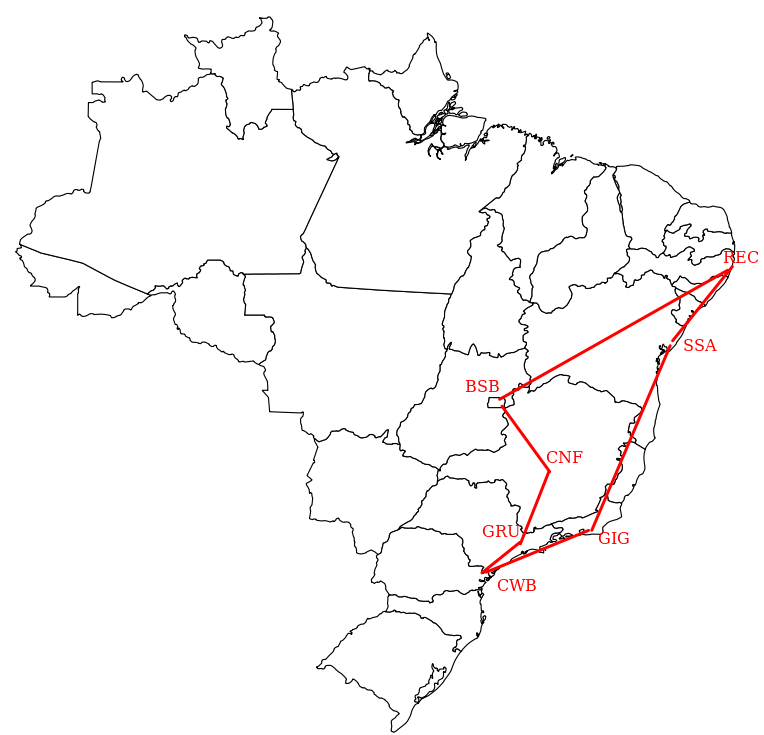
\includegraphics[scale=0.25]{Images/nodes.png}
		\captionof{figure}{A route between Brazilian airports}
		\label{fig:nodes}		
	\end{minipage}
\end{table}


In the {\it Brazilian Air Force}\/ missions, hundreds of items can be carried at each node, where the objectives are to prioritize the transport of the most important items and minimize the cost of fuel along the route. As standardized pallets are used with predefined positions on the aircraft, it is possible to carry out loading and unloading at each node in around two hours. However, there is no technological assistance that guarantees the achievement of these objectives.

\cite{MesquitaSanches2023} proposed a method that attends these objectives: a pallet building and arrangement plan with a routing option that maximizes the benefit-cost ratio for the smooth execution of pickup and delivery transport missions. They develop a heuristic that can be executed on a simple handheld computer (like a laptop or a tablet) and that provides a solution quickly enough to keep this cargo handling time under an hour.

In this work, we raise three hypotheses for improvements to the work of \cite{MesquitaSanches2023}:
(1) Computer parallelism could improve {\it Shims}'s performance.
(2) The {\it Shims}' results may have been inferior to that; it could be that a sequential approach to pallet building may lead to a premature stop due to the torque constraints.
(3) The distances to move pallets on unloading in the next node could be minimized to benefit unloading costs.

So, this work seeks to improve their results in terms of quality and performance by using computer parallelism, CG balancing between {\it Shims}' phases, and minimizing the distance between the next node-destined pallets and the cargo door.

These improvements in their heuristics are meant to reduce the stress that transport planners are subjected to, because they have to deal with a lot of information in planning the aircraft route, assembling the pallets, and picking up and delivering at each node. To the best of our knowledge, that is the first time that an air cargo transport problem that simultaneously involves APP, WBP, PDP and TSP has been addressed, and the first time ACLP+RPDP is solved with computer parallelism.

This article is organized into six more sections. In Section \ref{sec2}, we give a brief review of the literature. In Section \ref{sec3}, we present the problem context and assumptions and, in Section \ref{sec4}, the mathematical model and how we dealt with its issues. In Section \ref{sec5}, we describe the elaborate algorithms, whose results are presented in Section \ref{sec6}. Finally, our conclusions are in Section \ref{sec7}.


\section{Related literature}
\label{sec2}

In this section, we briefly describe the characteristics of the main works related to air cargo transport, following the chronological order of Table \ref{tab:sa}.

\cite{LarsenMikkelsen1979} developed an interactive procedure for loading 14 types of Boeing 747 into a two-leg flight plan. Seven types of items were considered to be allocated in 17 to 42 positions. With non-linear programming and heuristics, they present a solution that minimizes positioning changes in the intermediate node, optimizing the load balancing in the aircraft.

\cite{Brosh1981} addressed the problem of planning the allocation of cargo on an aircraft. Considering volume, weight and structural constraints, the author finds the optimal load layout through a fractional programming problem.

\cite{Kevin1992} developed a multi-criteria optimization approach to load the {\it C-130} aircraft of the {\it Canadian Air Force}. Based on integer programming, this model provides timely planning and improves airlift support for combat operations, solving WBP with pallets in fixed positions, and considering 20 different items.

\cite{Heidelberg1998} developed a heuristic for 2D packing in air loading, comparing it with methods for solving the {\it Bin Packing Problem}. Authors conclude that the classical algorithms are inadequate in this context, because they ignore the aircraft balancing constraints.

\cite{MongeauBes2003} presented a method based on linear integer programming to solve the problem of choosing and positioning containers on the {\it Airbus 340-300}. Safety and stability constraints were considered, with the objective of minimizing fuel consumption.

\cite{fok2004optimizing} developed a web-based application to make efficient use of space and load balancing for an air cargo company. Based on an analysis of historical data, an operational load planning with mathematical optimization is obtained. This container load planning is usually done roughly 2 hours before departure, when all cargo details are in place.

\cite{Chan2006} carried out a case study with heterogeneous pallets. In order to minimise the total cost of shipping, they developed a 3D packing heuristic, with a loading plan for each pallet. Although the authors do not consider load balancing or positioning of pallets in the cargo hold, this method is relevant in commercial and industrial applications, where cargo items tend to be less dense.

\cite{KaluznyBohdanL2009Oalb} developed a mixed integer linear programming model to arrange a set of items in a military context that optimizes the load balance.

\cite{Verstichel2011} solved WBP by selecting the most profitable subset of containers to be loaded onto an aircraft using mixed-integer programming. Experimental results on real-life data showed significant improvements compared to those obtained manually by an experienced planner.

\cite{MesquitaCunha2011} presented a heuristic for a real problem of the {\it Brazilian Air Force}, which consists of defining transport routes with simultaneous collection and delivery from a central distribution terminal. They used the {\it Scatter Search} metaheuristic as solution method.

\cite{Limbourg2012} developed a mixed-integer program for optimally rearranging a set of pallets into a compartmentalized cargo aircraft, specifically the {\it Boeing 747}.

\cite{kaspi2019} define and solve a new extension of the TSP to maximize the financial contribution per invested time and present an optimal iterative solution procedure for the problem which converges after a limited number of iterations.

\cite{RoesenerHall2014} solved APP and WBP as an integer programming problem, which also allows items to be loaded into pallets according to a specific orientation (e.g., this side up).

\cite{Vancroonemburg2014} presented a mixed integer linear programming model that selects the most profitable pallets, satisfying safety and load balancing constraints on the {\it Boeing 747-400}. Using a solver, authors solved real problems in less than an hour.

As already mentioned, \cite{LurkinSchyns2015} was the first work that simultaneously modeled WBP and SPDP in air cargo transport. The authors demonstrated that this problem is NP-hard and performed some experiments with real data, noting that their model offers better results than those obtained manually.

\cite{RoesenerBarnes2016} proposed a heuristic to solve the {\it Dynamic Airlift Loading Problem} (DALP). Given a set of palletized cargo items that require transport between two nodes in a time frame, the objective of this problem is to select an efficient subset of aircraft, partition the pallets into aircraft loads and assign them to allowable positions on those aircraft.

\cite{PaquaySchynsLimbourg2016} presented a mathematical modeling to optimize the loading of heterogeneous 3D boxes on pallets with a truncated parallelepipeds format. Its objective is to maximise the volume used in containers, considering load balancing constraints, the presence of fragile items and the possibility of rotating these boxes. \cite{PaquayLimbourgSchynsOliveira2018} developed some heuristics to solve this problem.

\cite{YangLiuGao2018} modelled the air transport problem as a 2D packing problem, and presented a heuristic for its optimization in several aircraft, considering load balancing in order to minimise fuel consumption.

\cite{wong2020}A developed a mathematical model and a tool based on mixed integer programming for optimizing cargo in aircraft with different pallet configurations. Balance constraints and the presence of dangerous items were considered. \cite{eugene2021} integrated this tool to a digital simulation model, with a visualization and validation system, based on sensors that alert about load deviations.

\cite{zhao2021} proposed a new modelling for WBP based on mixed integer programming. Instead of focusing on the center of gravity (CG) deviation, the authors consider the original CG envelope of the aircraft, with a linearization method for its non-linear constraints.

\cite{MesquitaSanches2023} contributed with a complex model and elaborate heuristics for the ACLP-RPDP that simultaneously solve 4 intractable sub-problems: APP, WBP, SPDP and TSP. They also compare the performances of four well known heuristics: {\it Ant Colony Optimization}, the {\it Noising Method Optimization}, the {\it Greedy Randomized Adaptive Search Procedure}, and {\it Tabu Search}. They also create a new heuristic called {\it Shims} which is fast and may be run in a handheld computer. They did not use computer parallelism to improve performance, nor tryed to minimize the distances from the next nodes destined pallets to the cargo ramp door.

As can be seen, except for \cite{MesquitaSanches2023}, the remaining works do not address air cargo palletization and load balancing with route optimization in a multi-leg flight plan, and none of them employ parallelization in their algorithms. This is the objective of our work: to reshape \cite{MesquitaSanches2023} solution process and algorithms to accommodate parallel features that can improve solution quality and performance, and also include a new feature that is to minimize the distances between the next node's destined pallets and the cargo ramp door.


\section{Problem context and assumptions}
\label{sec3}

In this section, we describe the context of the problem addressed in this work, as well as the assumptions considered.

\subsection{Operational premises}

As we are dealing with an extremely complex and diverse problem, we decided to establish some simplifying characteristics:

\begin{itemize}
	
	\item At each node of the flight plan, the items to be allocated are characterized by weight, volume, scores, and previously known destinations, but do not have dimensions. We leave the consideration of 2D or 3D items for future work.
	
	\item We also disregarded {\it hazardous} items, which eventually could be treated as high score items and other specific constraints.
	
	\item We considered a unique pallet type: the {\it 463L Master Pallet}, a common size platform for bundling and moving air cargo. It is the primary air cargo pallet for more than 70 Air Forces and many air transport companies. This pallet has a capacity of $4500 kg$ and $14.8 m^3$, is equipped for locking into cargo aircraft rail systems, and includes tie-down rings to secure nets and cargo loads, which in total weighs $140 kg$. For more information, see {\tt www.463LPallet.com}.
	
	\item All items allocated on a pallet must have the same destination. A pallet which has not yet reached its destination may receive more items, although it is known that these operations of removing restraining nets increase handling time and the risk of improper delivery. We do not consider oversized cargo in this work, but only cargoes that fit on these pallets.
	
	\item Pallets with destinations set to the next node should be put as near as possible to the cargo ramp door.

	\item Finally, as we are interested in minimizing fuel costs while keeping the CG in its operational range, we disregarded some lower ones as handling costs.

\end{itemize}

Throughout this text, we call a {\it consolidated item} a set of items of the same destination stacked on a pallet and covered with a restraining net. It is considered unique, having the same attributes of its components, whose values are the sum of individual scores, weights and volumes. See Figure \ref{fig:larger2}.
Consolidated items must stay on board until they reach their destination to maintain accuracy in pickup and delivery procedures.


\begin{figure}[H]
	\centering
	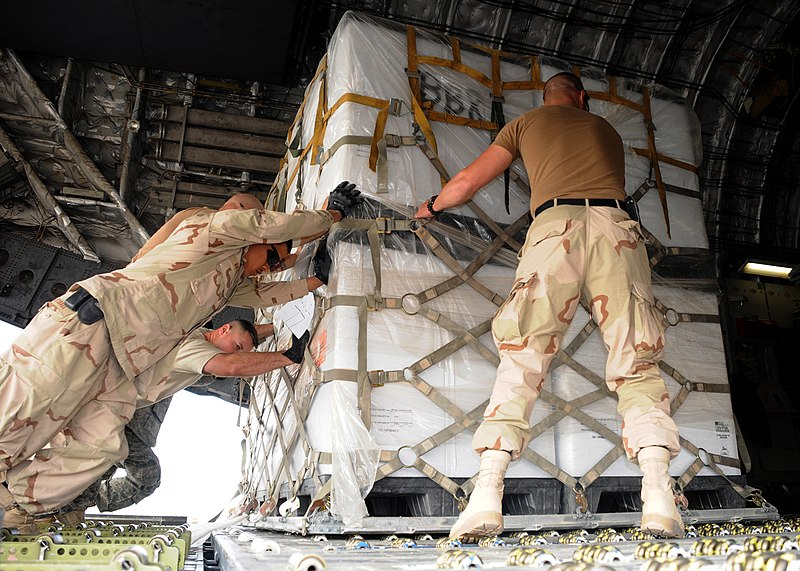
\includegraphics[scale=0.4]{Images/consolidated.jpg}
	\caption{Consolidated items on 463L pallets inside a {\it Boeing C-17}}
	\small\textsuperscript{Source: From Wikimedia Commons, the free media repository}
	\label{fig:larger2}
\end{figure}



\subsection{Aircraft and load balancing}


We consider real scenarios with a smaller or a larger aircraft with payloads of 26,000 kg or 75,000 kg respectively. Both layouts are represented in Figures \ref{fig:smaller} and \ref{fig:larger}, where the pallets are identified by $p_i$.

\begin{figure}[!h]
	\centering
	
	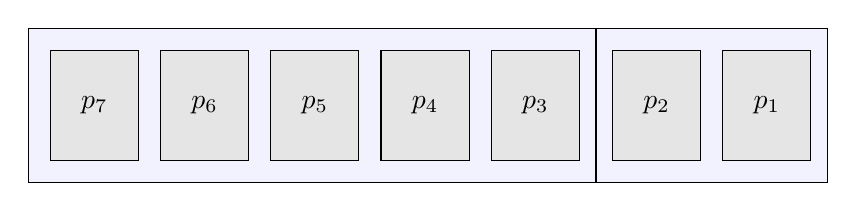
\begin{tikzpicture}[scale=1.4, samples=100]
		
		\filldraw[fill=blue!5!white, draw=black] (0, 0) rectangle (5.15, 1.4);
		\filldraw[fill=gray!20!white, draw=black] (0.2, 0.2) rectangle node{$p_7$} (1.0, 1.2); 
		\filldraw[fill=gray!20!white, draw=black] (1.2, 0.2) rectangle node{$p_6$} (2.0, 1.2); 
		\filldraw[fill=gray!20!white, draw=black] (2.2, 0.2) rectangle node{$p_5$} (3.0, 1.2); 
		\filldraw[fill=gray!20!white, draw=black] (3.2, 0.2) rectangle node{$p_4$} (4.0, 1.2); 
		\filldraw[fill=gray!20!white, draw=black] (4.2, 0.2) rectangle node{$p_3$} (5.0, 1.2); 
		\filldraw[fill=blue!5!white,  draw=black] (5.15,  0) rectangle             (7.25, 1.4);
		\filldraw[fill=gray!20!white, draw=black] (5.3, 0.2) rectangle node{$p_2$} (6.1, 1.2); 
		\filldraw[fill=gray!20!white, draw=black] (6.3, 0.2) rectangle node{$p_1$} (7.1, 1.2);	
		
	\end{tikzpicture}
	
	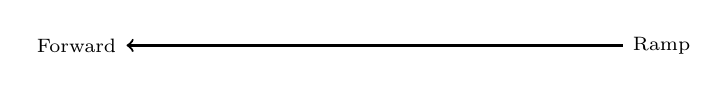
\begin{tikzpicture}[scale=1.4, samples=100]
		\draw[black, thick][<-]  (1, 2.17) node[anchor=east, font=\fontsize{7}{3.5}\selectfont]{Forward} -- (5.5, 2.17) node[anchor=west, font=\fontsize{7}{3.5}\selectfont]{Ramp} ;
	\end{tikzpicture}
	
	\caption{Smaller aircraft layout}
	%\small\textsuperscript{Source: the author}	
	\label{fig:smaller}
\end{figure}

\begin{figure}[!h]
	\centering
	
	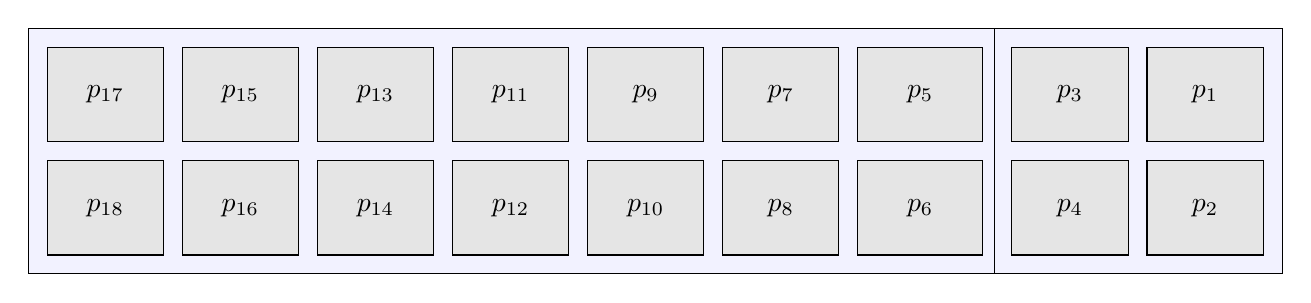
\begin{tikzpicture}[scale=1.2, samples=100]
		
		\filldraw[fill=blue!5!white, draw=black] (0, 0) rectangle (10.23, 2.6);
		
		\filldraw[fill=gray!20!white, draw=black] (0.20, 1.40) rectangle node{$p_{17}$} (1.43, 2.40);
		\filldraw[fill=gray!20!white, draw=black] (0.20, 0.20) rectangle node{$p_{18}$} (1.43, 1.20);
		
		\filldraw[fill=gray!20!white, draw=black] (1.63, 1.40) rectangle node{$p_{15}$} (2.86, 2.40);
		\filldraw[fill=gray!20!white, draw=black] (1.63, 0.20) rectangle node{$p_{16}$} (2.86, 1.20);
		
		\filldraw[fill=gray!20!white, draw=black] (3.06, 1.40) rectangle node{$p_{13}$} (4.29, 2.40);
		\filldraw[fill=gray!20!white, draw=black] (3.06, 0.20) rectangle node{$p_{14}$} (4.29, 1.20);
		
		\filldraw[fill=gray!20!white, draw=black] (4.49, 1.40) rectangle node{$p_{11}$} (5.72, 2.40);
		\filldraw[fill=gray!20!white, draw=black] (4.49, 0.20) rectangle node{$p_{12}$} (5.72, 1.20);
		
		\filldraw[fill=gray!20!white, draw=black] (5.92, 1.40) rectangle node{$p_{9}$} (7.15, 2.40);
		\filldraw[fill=gray!20!white, draw=black] (5.92, 0.20) rectangle node{$p_{10}$} (7.15, 1.20);
		
		\filldraw[fill=gray!20!white, draw=black] (7.35, 1.40) rectangle node{$p_{7}$} (8.58, 2.40);
		\filldraw[fill=gray!20!white, draw=black] (7.35, 0.20) rectangle node{$p_{8}$} (8.58, 1.20);
		
		\filldraw[fill=gray!20!white, draw=black] (8.78, 1.40) rectangle node{$p_{5}$} (10.1, 2.40);
		\filldraw[fill=gray!20!white, draw=black] (8.78, 0.20) rectangle node{$p_{6}$} (10.1, 1.20);
		
		\filldraw[fill=blue!5!white, draw=black] (10.23, 0) rectangle (13.27, 2.6);
		\filldraw[fill=gray!20!white, draw=black] (10.41, 1.40) rectangle node{$p_{3}$} (11.64, 2.40);
		\filldraw[fill=gray!20!white, draw=black] (10.41, 0.20) rectangle node{$p_{4}$} (11.64, 1.20);
		\filldraw[fill=gray!20!white, draw=black] (11.84, 1.40) rectangle node{$p_{1}$} (13.07, 2.40);
		\filldraw[fill=gray!20!white, draw=black] (11.84, 0.20) rectangle node{$p_{2}$} (13.07, 1.20);
		
	\end{tikzpicture}
	
	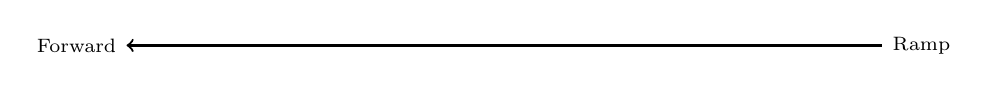
\begin{tikzpicture}[scale=1.2, samples=100]
		\draw[black, thick][<-]  (1, 2.77) node[anchor=east, font=\fontsize{7}{3.5}\selectfont]{Forward} -- (9, 2.77) node[anchor=west, font=\fontsize{7}{3.5}\selectfont]{Ramp} ;
	\end{tikzpicture}
	
	
	\caption{Larger aircraft layout} \label{fig:larger}
\end{figure}

In both cases, the torque applied to the aircraft must keep its CG in the operational range, which corresponds to a percentage of the {\it Mean Aerodynamic Chord} \footnote{Chord is the distance between the leading and trailing edges of the wing, measured parallel to the normal airflow over the wing \cite[p.18]{HoughtonCarpenter2003}. The average length of the chord is known as the {\it Mean Aerodynamic Chord} (MAC).}: $0.556m$ in the smaller aircraft and $1.17m$ in the larger one. See Figure \ref{fig:lateral}.

\begin{figure}[H]
	\centering
	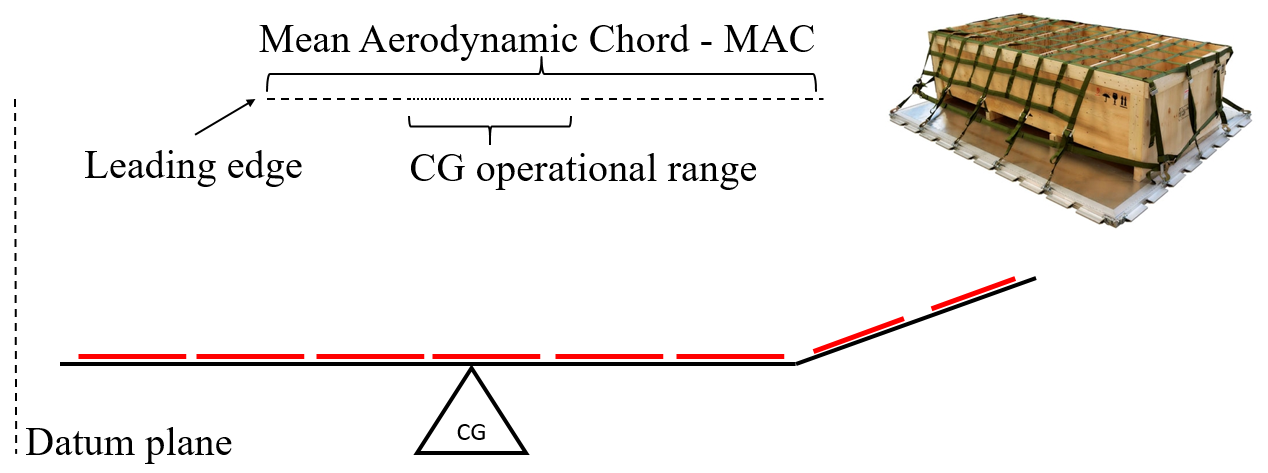
\includegraphics[scale=0.24]{Images/lateral.png}
	\caption{Aircraft longitudinal cut showing red lines as pallets}
	%\small\textsuperscript{Source: the author}
	\label{fig:lateral}
\end{figure}

Tables \ref{tab:smaller} and \ref{tab:larger} show the parameters in both cases. {\it CGx} and {\it CGy} refer to the relative distances of pallet centroids (in meters) in relation to the CG of aircraft along both axes. In both aircraft, as the ramps have an inclination of 25 degrees, we made the necessary corrections in {\it CGx}, {\it Weight} and {\it Volume limits} of the corresponding pallets. The monetary costs of both aircraft are also indicated: per unit of distance in flights between legs ($c_d$) and per deviation in the CG ($c_g$). It is important to consider that $c_g$ tends to zero as the aircraft attitude tends to level.


\begin{table}[H]
	\centering
	\caption{Smaller aircraft parameters}  \label{tab:smaller}
	\footnotesize
	\begin{tabular}{c | c c c c c c c}
		\toprule
		\bf {Limits}  & \multicolumn{3}{c}{$Payload$: $26,000kg$} & \multicolumn{4}{c}{$limit^{CG}_{long}$: $0.556m$} \\
		\midrule
		\bf {Pallets} & $p_7$ & $p_6$ & $p_5$ & $p_4$ & $p_3$ & $p_2$ & $p_1$ \\
		\midrule
		{\bf CGx ($m$)}     & -5.10 & -2.70 & -0.30   & 2.10 & 4.50 & 6.25 & 8.39  \\
		\midrule
		{\bf Weight limits ($kg$)}  & 4,500  &  4,500 &  4,500   & 4,500 & 4,500 & 4,000 & 3,500 \\ 
		{\bf Volume limits ($m^3$)} & 13.7  &  13.7 &  13.7   & 13.7 & 13.7 & 8.9 & 6.9 \\ 
		\midrule

		\bf {Costs}  & \multicolumn{4}{c}{$c_d$: US\$ $1.100/km$ } &	\multicolumn{3}{c}{$c_g = 0.05$} \\

		\bottomrule
	\end{tabular}
	\normalsize 
\end{table}


\begin{table}[H]
	\centering
	\caption{Larger aircraft parameters}  \label{tab:larger}
	\footnotesize
	\begin{tabular}{c | c c c c c c c c c}
		\toprule
		\bf {Limits}& \multicolumn{3}{c}{$Payload$: $75,000kg$} & \multicolumn{3}{c}{$limit^{CG}_{long}$: $1.170m$} &
		\multicolumn{3}{c}{$limit^{CG}_{lat}$: $0.19m$} \\
		\midrule
		\multirow{2}{*}{\bf {Pallets}}  & $p_{17}$ & $p_{15}$ & $p_{13}$ & $p_{11}$ & $p_{9}$ & $p_{7}$ & $p_{5}$ & $p_{3}$ & $p_{1}$ \\
		& $p_{18}$ & $p_{16}$ & $p_{14}$ & $p_{12}$ & $p_{10}$ & $p_{8}$ & $p_{6}$ & $p_{4}$ & $p_{2}$ \\
		\midrule 
		\multirow{2}{*}{\bf {CGx ($m$)}} & -17.57 & -13.17 & -8.77 & -4.40 & 0 & 4.40 & 8.77 & 11.47 & 14.89 \\
		& -17.57 & -13.17 & -8.77 & -4.40 & 0 & 4.40 & 8.77 & 11.47 & 14.89 \\			
		\midrule 
		\multirow{2}{*}{\bf {CGy ($m$)}}  & 1.32 & 1.32 & 1.32 & 1.32 & 1.32 & 1.32 & 1.32 & 1.32 & 1.32 \\
		& -1.32 & -1.32 & -1.32 & -1.32 & -1.32 & -1.32 & -1.32 & -1.32 & -1.32 \\	
		\midrule
		{\bf Weight limits ($kg$)}      &   4,500   &    4,500  &   4,500   &  4,500    & 4,500     & 4,500     & 4,500     & 4,000    & 3,000   \\
		{\bf Volume limits ($m^3$)}   &   14.8   &   14.8   &  14.8    &  14.8    & 14.8     & 14.8     & 14.8     & 10.0    & 7.0 \\	
		\midrule	

		\bf {Costs}  & \multicolumn{5}{c}{ $c_d$: US\$ $4.900/km$ } &	\multicolumn{4}{c}{$c_g = 0.05$} \\

		\bottomrule
	\end{tabular}
	\normalsize 
\end{table}

We accept the same assumptions as stated by \cite{MesquitaSanches2023}:
\begin{itemize}
	\item on each pallet, the items are distributed in such a way that their CG coincides with the centroid of the pallet;
	\item the CG of the payload must be at a maximum longitudinal distance of $limit^{CG}_{long}$ from the CG of the aircraft;
	\item in the larger aircraft, the CG of the payload must be at a maximum lateral distance of $limit^{CG}_{lat}$ from the CG of the aircraft;
	\item in the larger aircraft, pallets are distributed in two identical rows (with odd and even indices, respectively), and their centroids are at a distance $d^{CG}_{pallet}$ from the center-line of the aircraft.
\end{itemize}

\subsection{Problem Summary}

\newcolumntype{M}{>{\raggedright}p{0.03\textwidth}}
\newcolumntype{T}{>{\raggedright\arraybackslash}p{0.9\textwidth}}

\bgroup
\def\arraystretch{1.2}
\begin{table}[H]
	\centering
	\small
	\begin{tabular}{MT}
		&Informally, ACLP+RPDP can be summarized as follows:\\
		\midrule
		max &  (items score sum) / (tour cost) of picked up and delivered items on a tour  \\
		\midrule
s.t.    & Along a tour, the set of unvisited nodes is updated. \\
		& In each node, an item may be included in at most one pallet.\\		
		& In each node, consolidated items are composed of items with the same destination. \\
		& Weight, volume and score of a consolidated item are the corresponding sum of their components.\\
		& Consolidated items remain on board until their destinations.\\	
		& Consolidated items can only be included in the same pallet if their destinations are the same.\\
		& Only items destined for the remaining nodes can be loaded.  \\
		& The lateral and longitudinal torques must be within the operational range of the aircraft.\\
		& Weight and volume limitations of pallets must be respected.\\
		& The total weight must be less than the aircraft payload or the total pallet capacity, whichever is the lowest.\\	
		& {\bf The pallets destined for the next node of the tour should be put as near as possible to the cargo ramp door (our inclusion)}.\\		
		\midrule
	\end{tabular}
	\normalsize
\end{table}
\egroup 


\section{The mathematical modelling}
\label{sec4}

Given the assumptions, scenarios and parameters described in the previous section, we are ready to present the mathematical modelling of ACLP+RPDP.

Let $L = \{ l_0, l_1, \ldots, l_K \}$ be the set of $K+1$ nodes (or destinations), where $l_0$ is the origin and end of a flight plan. Let $d(l_i,l_j)$ be the distance from $l_i$ to $l_j$, where $0 \leq i,j \leq K$. By definition, $d(l_i,l_i)=0$. Let $L_k$ be the set of remaining nodes when the aircraft is in $l_k$, $0 \leq k \leq K$. Therefore, $L_0=L$ and $L_K = \{ l_0 \}$.

Let $C=\{c_{ij}\}$ be the cost matrix of flights, where $c_{ij} = c_d*d(l_i,l_j), 0 \leq i,j \leq K$.

Let $S_K = \{s: \{1, \dots, K\} \rightarrow \{1, \dots, K\} \}$ be the set of $K!$ permutations, which correspond to all possible tours (or itineraries) that have $l_0$ as origin and end, passing through the other $K$ nodes. {\color{blue} $k$ is the node index and $\pi(k)$ is the node in position $k$ of tour $\pi$}.

Let $M = \{p_1, p_2, \ldots, p_m \}$ the set of $m$ pallets. Each pallet $p_i$, $1 \leq i \leq m$, has weight capacity $p_i.w$, volume capacity $p_i.v$, pallet destinations $p_i.to[{\pi(k)}]$, $0 \leq k \leq K$, and distance to the CG of aircraft $p_i.d$. $p_i.to[{\pi(k)}]$ denotes that pallet $p_i$ may assume a different destination in each node ${\pi(k)}$.

Let $N_{\pi(k)} = \{t^{\pi(k)}_1, t^{\pi(k)}_2, \ldots, t^{\pi(k)}_{n_{\pi(k)}} \}$ be the set of $n_{\pi(k)}$ items to be loaded in node $l_{\pi(k)}$, $0 \leq k \leq K$. Each item $t^{\pi(k)}_j$, $1 \leq j \leq n_{\pi(k)}$, has score $t^{\pi(k)}_j.s$, weight $t^{\pi(k)}_j.w$, volume $t^{\pi(k)}_j.v$, and destination $t^{\pi(k)}_j.to \in L_{\pi(k)}$. Let $N = \bigcup_{0 \leq k \leq K} N_{\pi(k)}$ be the set of items of all nodes along a tour.

Let $Q_{\pi(k)} = \{a^{\pi(k)}_1, a^{\pi(k)}_2, \ldots, a^{\pi(k)}_{m_{\pi(k)}} \}$ be the set of consolidated items loaded in $m_k \leq m$ pallets when the aircraft arrives at node $l_{\pi(k)}$, with $0 \leq k \leq K$. $a^{\pi(k)}_i$, $1 \leq i \leq m_{\pi(k)}$, is the group of picked-up items that were allocated on pallet $p_i$ in some of the previous nodes. $a^{\pi(k)}_i$ has total weight $a^{\pi(k)}_i.w$, total volume $a^{\pi(k)}_i.v$, and destination $a^{\pi(k)}_i.to \in L_{\pi(k)} \cup \{l_{\pi(k)}\}$. If $a^{\pi(k)}_i.to = l_{\pi(k)}$, then $a^{\pi(k)}_i$ is unloaded, and $p_i$ will be available for reloading; otherwise, $a^{\pi(k)}_i$ remains on the aircraft, eventually in another pallet, and with items of $N_{\pi(k)}$ having the same destination.

Let $X_{ij}^{\pi(k)}$ and $Y_{iq}^{\pi(k)}$ be binary variables, where $0 \leq k \leq K$, $1 \leq j \leq n_{\pi(k)}$, $1 \leq i \leq m$ and $1 \leq q \leq m_{\pi(k)}$. $X_{ij}^{\pi(k)} = 1$ if $t_j^{\pi(k)}$ is assigned to $p_i$ in node $l_{\pi(k)}$, and 0 otherwise. $Y_{iq}^{\pi(k)} = 1$ if $a_q^{\pi(k)}$ is assigned to $p_i$ in node $l_{\pi(k)}$, and 0 otherwise. By definition, $Y_{iq}^0=0$. Allocations of items or consolidated items to pallets in node $l_{\pi(k)}$ can be seen as a bipartite graph $G_{\pi(k)}(V_{\pi(k)}, E_{\pi(k)})$, where $V_{\pi(k)} = M \cup N_{\pi(k)} \cup Q_{\pi(k)}$, $E_{\pi(k)} = E^N_{\pi(k)} \cup E^Q_{\pi(k)}$, $(p_i, t_j^{\pi(k)}) \in E^N_{\pi(k)}$ if $X_{ij}^{\pi(k)} = 1$, and $(p_i, a_q^{\pi(k)}) \in E^Q_{\pi(k)}$ if $Y_{iq}^{\pi(k)} = 1$.

The mathematical modeling of this problem is described in the equations below.


\begin{equation} \label{eq:maxf}
	\max_{\pi \in S_K} f_\pi(\tilde{s},\tilde{c})
\end{equation}

\begin{equation} \label{eq:scores}
	\tilde{s} = \sum_{k=0}^{K} \sum_{i=1}^{m} \sum_{j=1}^{n_{\pi(k)}} X_{ij}^{\pi(k)} \times t_j^{\pi(k)}.s
\end{equation}

\begin{equation} \label{eq:costs}
	\tilde{c} = c_{0,\pi(1)}\times(1+c_g\times|\epsilon_0|) + \sum_{k=1}^{K-1} [ c_{\pi(k), \pi(k+1)}\times(1+c_g\times|\epsilon_{\pi(k)}|) ] + c_{\pi(K),0}\times(1+c_g\times|\epsilon_K|)
\end{equation}

\begin{equation} \label{eq:maxW}
	maxW = \min(Payload, \sum_{i=1}^{m}p_i.w)
\end{equation}

\begin{equation} \label{eq:tau}
\tau_{\pi(k)} = \sum_{i=1}^{m}[ p_i.d \times (\sum_{j=1}^{n_{\pi(k)}} X_{ij}^{\pi(k)} \times t_j^{\pi(k)}.w +  \sum_{q=1}^{m} Y_{iq}^{\pi(k)} \times a_q^{\pi(k)}.w)];\ k \in \{0, 1, \ldots, K\}
\end{equation}

\begin{equation} \label{eq:eps}
\epsilon_{\pi(k)} = \frac{\tau_{\pi(k)}}{maxW \times limit^{CG}_{long}};\ k \in \{0, 1, \ldots, K\}
\end{equation}

\begin{equation} \label{eq:pdp11}
	L_0 = L; L_{\pi(k)} = L_{{\pi(k-1)}} - \{l_{\pi(k)}\}; \ k \in \{1, 2, \ldots, K\}
\end{equation}

\begin{equation} \label{eq:pdp13}
	Y^0_{iq} = 0; a^0_i.w = 0; a^0_i.v = 0; a^0_i.to = -1;\ i,q \in \{1, 2, \ldots, m\}
\end{equation}

\begin{equation} \label{eq:pdp12}
	X_{ij}^{\pi(k)} = 0 \ \mbox{if} \ t_j^{\pi(k)}.to \notin L_{\pi(k)}; \ i \in \{1, 2, \ldots, m\}; \ j \in \{1, 2, \ldots, n_{\pi(k)}\}; \ k \in \{1,2, \ldots, K\}
\end{equation}

\begin{equation} \label{eq:pdp9}
	Y_{iq}^{\pi(k)} = 0 \ \mbox{if} \ a_i^{\pi(k)}.to \notin L_{\pi(k)}; \ i \in \{1, 2, \ldots, m\}; \ q \in \{1, 2, \ldots, m_{\pi(k)}\}; \ k \in \{ 1, 2, \ldots, K\}
\end{equation}

\begin{equation} \label{eq:cons2}
	a_i^{\pi(k+1)}.w = \sum_{j=1}^{n_{\pi(k)}} X_{ij}^{\pi(k)} \times t_j^{\pi(k)}.w + \sum_{q=1}^{m_{\pi(k)}} Y_{iq}^{\pi(k)} \times a_q^{\pi(k)}.w;  \ i \in \{1, 2, \ldots, m_{\pi(k)}\}; k \in \{0, 1, \ldots, K-1\}
\end{equation}

\begin{equation} \label{eq:cons3}
	a_i^{\pi(k+1)}.v = \sum_{j=1}^{n_{\pi(k)}} X_{ij}^{\pi(k)} \times t_j^{\pi(k)}.v + \sum_{q=1}^{m_k} Y_{iq}^{\pi(k)} \times a_q^{\pi(k)}.v;  \ i \in \{1, 2, \ldots, m_{\pi(k)}\}; k \in \{0, 1, \ldots, K-1\}
\end{equation}

\begin{equation} \label{eq:cons5}
	a_i^{\pi(k+1)}.to = t^{\pi(k)}_j.to  \ \mbox{if} \ X^{\pi(k)}_{ij} = 1  \ \mbox{and} \ t^{\pi(k)}_j.to \in L_{\pi(k+1)};  \ i \in \{1, 2, \ldots, m_{\pi(k)}\}; \ j \in \{1, 2, \ldots, n_{\pi(k)}\}; \ k \in \{0,1, \ldots, K-1\}
\end{equation}

\begin{equation} \label{eq:LatIt}
	LatIt_{\pi(k)} = \sum_{i=1}^{m} \sum_{j=1}^{n_{\pi(k)}} ( X_{ij}^{\pi(k)} \times t_j^{\pi(k)}.w \times (i\%2) - X_{ij}^{\pi(k)} \times t_j^{\pi(k)}.w \times (i+1)\%2 ); \ k \in \{0, 1, \ldots, K\}
\end{equation}

\begin{equation} \label{eq:LatCons}
	LatCons_{\pi(k)} =  \sum_{i=1}^{m} \sum_{q=1}^{m_{\pi(k)}}  ( Y_{iq}^{\pi(k)} \times a_q^{\pi(k)}.w \times (i\%2) - Y_{iq}^{\pi(k)} \times a_q^{\pi(k)}.w \times (i+1)\%2); \ k \in \{0, 1, \ldots, K\}
\end{equation}

\begin{equation} \label{eq:torqlat}
	s.t.: d^{CG}_{pallet} \times | LatIt_{\pi(k)} + LatCons_{\pi(k)} | \leq  \sum_{i=1}^{m}p_i.w \times limit^{CG}_{lat}; \ k \in \{0, 1, \ldots, K\}
\end{equation}

\begin{equation} \label{eq:torqlong}
	s.t.: |\tau_{\pi(k)}| \leq maxW \times limit^{CG}_{long};\ k \in \{0, 1, \ldots, K\}
\end{equation}

\begin{equation} \label{eq:payload}
	s.t.: \sum_{i=1}^{m} (\sum_{j=1}^{n_{\pi(k)}} X_{ij}^{\pi(k)} \times t_j^{\pi(k)}.w + \sum_{q=1}^{m_k} Y_{iq}^{\pi(k)} \times a_q^k.w ) \leq maxW; \ k \in \{0, 1, \ldots, K\}
\end{equation}

\begin{equation} \label{eq:app2}
	s.t.: \sum_{j=1}^{n_{\pi(k)}} X_{ij}^{\pi(k)} \times t_j^{\pi(k)}.w + \sum_{q=1}^{m_k} Y_{iq}^{\pi(k)} \times a_q^{\pi(k)}.w  \leq p_i.w; \ i \in \{1, 2, \ldots, m_{\pi(k)}\}; \ {\pi(k)} \in \{0, 1, \ldots, K\}
\end{equation}

\begin{equation} \label{eq:app3}
	s.t.: \sum_{j=1}^{n_{\pi(k)}} X_{ij}^{\pi(k)} \times t_j^{\pi(k)}.v + \sum_{q=1}^{m_{\pi(k)}} Y_{iq}^{\pi(k)} \times a_q^{\pi(k)}.v  \leq\ p_i.v; \ i \in \{1, 2, \ldots, m_{\pi(k)}\}; \ k \in \{0, 1, \ldots, K\}
\end{equation}

\begin{equation} \label{eq:app4}
	s.t.: \sum_{i=1}^{m} X_{ij}^{\pi(k)} \leq 1; \ j \in \{1, 2, \ldots, n_{\pi(k)}\}; \ k \in \{0, 1, \ldots, K\}
\end{equation}

\begin{equation} \label{eq:app5}
	s.t.:  Y_{iq}^{\pi(k)} = 1 \ \mbox{if} \ a^{\pi(k)}_q.to \in L_{\pi(k)}; \ q \in \{1, 2, \ldots, m_{\pi(k)}\}; \ k \in \{0, 1, \ldots, K\}
\end{equation}

\begin{equation} \label{eq:pdp8}
	s.t.: p_i.to[{\pi(k)}] = t^{\pi(k)}_j.to\ \mbox{if} \ X_{ij}^{\pi(k)} = 1; \ i \in \{1, 2, \ldots, m\}; \ j \in \{1, 2, \ldots, n_{\pi(k)}\}; \ k \in \{1, 2, \ldots, K\}
\end{equation}

\begin{equation} \label{eq:pdp2}
	s.t.:  p_i.to[{\pi(k)}] = a^{\pi(k)}_q.to\ \mbox{if} \ Y_{iq}^{\pi(k)} = 1; \ i \in \{1, 2, \ldots, m\};\ q \in \{1, 2, \ldots, m_{\pi(k)}\}; \ k \in \{1, 2, \ldots, K\}
\end{equation}


The objective of this problem is to find a permutation $\pi \in S_K$\/ that maximizes the function $f_\pi(\tilde{s},\tilde{c})$ \ref{eq:maxf}. In this way, the flight plan will be $l_0, l_{\pi(1)}, \ldots, l_{\pi(K)}, l_0$. $\tilde{s}$\/ is the total score of transported items \ref{eq:scores} and  $\tilde{c}$\/ is the total cost of fuel consumed \ref{eq:costs}. As can be seen, $\tilde{c}$\/ corresponds to the fuel consumption due to the flights carried out and the CG deviation of the transported cargo. Throughout this work, for simplicity, we use $f=\tilde{s}/\tilde{c}$.

The maximum load will be the minimum between the payload and the capacity supported by the pallets \ref{eq:maxW}. Considering the maximum longitudinal distance allowed for the CG, all torques \ref{eq:tau} and deviations \ref{eq:eps} are calculated.

For each step of the flight plan, the set of unvisited nodes is updated \ref{eq:pdp11}. Although there are no items consolidated at the beginning of the flight plan, we defined these variables for ease of notation \ref{eq:pdp13}. Items destined outside the rest of the flight plan will not be loaded (\ref{eq:pdp12} and \ref{eq:pdp9}).

Consolidated items appear when there are items on the pallets that will not be unloaded on the next node. Its weights \ref{eq:cons2} and volumes \ref{eq:cons3} correspond to all the items that were on the pallet, since all these items have the same destination. On subsequent nodes, consolidated items can be allocated with other items of same destination \ref{eq:cons5}.

Equations \ref{eq:LatIt} and \ref{eq:LatCons} respectively, are applied only to the larger aircraft, and calculate the lateral torques of items and consolidated items loaded in both rows of pallets, whose constraint is described in \ref{eq:torqlat}. Similarly, \ref{eq:torqlong} is the longitudinal torque constraint, which is applied to both aircraft sizes.

The weight limitation of the aircraft must be respected \ref{eq:payload}. The sum of weights \ref{eq:app2} and volumes \ref{eq:app3} in each pallet must not exceed its capacity. Each item is associated with a pallet at most \ref{eq:app4}.

Consolidated items remain on board \ref{eq:app5} until their destinations. At each node, an item (\ref{eq:pdp8}) and a consolidated item (\ref{eq:pdp2}) must only be allocated to a pallet if the destinations are the same.


\section{Resolution strategy}
\label{sec5}

Once the assumptions of this work and the mathematical modelling of the problem are presented, it is easy to see that ACLP+RPDP is NP-hard. In a similar way to \cite[p. 6]{LurkinSchyns2015}, consider the simple case where $K=1$\/ (one leg), $m=2$ (two pallets around the aircraft CG), $2n$\/ sufficiently light items with same scores in $l_0$, and no items in $l_1$. Under these conditions, through polynomial reductions for the {\it Set-Partition Problem}, it is possible to demonstrate that the decision problem associated with ACLP+RPDP is NP-hard.

Real cases are more complex as they have hundreds of different items in each node and involve three intractable sub-problems: APP, WBP and SPDP. Through the mathematical modeling presented in the previous section, we verify that {\it Mixed-Integer Programming}\/ (MIP) is not able to solve these cases in feasible time. Thus, it is necessary to adopt some strategy to find a viable solution, not necessarily optimal, that seeks to maximize the objective function $f$.

\cite{MesquitaSanches2023} strategy is based on the fact that, in real cases, $K$\/ is usually small. Specifically, they will consider $K \leq 6$\/ throughout their and our work, which is a higher value than usual in {\it Brazilian Air Force} missions. As a result, if we have fast node-by-node solutions that allow us to construct a complete tour, we will be able to test all possible $K!$\/ tours and thus select the one that provides the best value for the $f$\/ function.

Each node, except the base, inherits information from the previous nodes (pallets that must remain on board), and must be solved taking into account the remaining not visited nodes. One more reason for a node-by-node approach.

The tactic will be, at each shipping node, to predefine the destinations of the pallets at that node. In this way, we will reserve a number of pallets proportional to the volume demanded by each destination at the shipping node. We could have used another criterion, but it was observed in the experiments that volume is more constrictive in airlift. Once the destinations of the pallets are defined, we will use serial and Multi-processing heuristics to find the best possible node-by-node solutions. This strategy is summarized in Algorithm \ref{alg:main}, retrieved from \cite{MesquitaSanches2023}.


\begin{algorithm}[H]
	\caption{Solves ACLP+RPDP for a scenario with certain volume surplus (1.2, 1.5, or 2.0)}  \label{alg:main}
	\begin{algorithmic}[1]
		
		\Procedure{$ACLP+RPDP$}{$scenario,\ surplus,\ timeLim$}
		
		\State Let $L, M, C$ be according to $scenario$ \label{main:LMC}
		\State $N \gets ItemsGeneration(scenario,\ surplus)$ \label{main:items}
		\For {each $method$}
				
			\For {each $\pi \in S_K$} \label{main:loop1}
				\State $f_{\pi} \gets SolveTour(\pi, L, M, C, N, method, \ timeLim )$ \label{main:method}
			\EndFor \label{main:loop2}
			\State $answer[scenario,surplus,method] \gets \max f$ \label{main:f}
		\EndFor
		
		\Return $answer$
		
		\EndProcedure
	\end{algorithmic}
\end{algorithm}


In this algorithm, there are six values for the $scenario$\/ parameter, according to Table \ref{tab:scenarios}, which defines $K$, the sets of nodes, the aircraft, the pallets and the costs from Tables \ref{tab:smaller} or \ref{tab:larger} that will be used (line \ref{main:LMC}).


The other parameter $volume$\/ is a value greater than 1, which corresponds, at each node $l_{\pi(k)}$, to the ratio between the sum of the volumes of the items ($\sum_{j=1}^{n_{\pi(k)}} t^{\pi(k)}_j.v$) and the load capacity of the pallets ($\sum_{i=1}^{m} p_i.v$). This parameter is passed to $ItemsGeneration$ (line \ref{main:items}), responsible for creating the items to be shipped, which will be presented in the next section.

$method$\/ corresponds to one of the heuristics that we will present in subsection \ref{methods}. The loop of lines \ref{main:loop1}-\ref{main:loop2} goes through all permutations $\pi$, where the node-by-node resolutions are performed by $SolveTour$, whose result is stored in $f_{\pi}$. The best result among all $K!$\/ tours will be the answer for $scenario$, $volume$\/ and $method$\/ (line \ref{main:f}). 

\vspace{2.0mm}
\begin{table}[H]
	\centering
	\caption{Testing scenarios retrieved from \cite{MesquitaSanches2023}.}  \label{tab:scenarios}
	\begin{tabular}{c c c c }
		\toprule
		{\bf Scenario} & {$K$} & {$L$} & {\bf Aircraft} \\		
		\midrule
		1 & 2    & \{$l_0$, $l_1$, $l_2$\}                                 & smaller \\
		2 & 2    & \{$l_0$, $l_1$, $l_2$\}                                 & larger  \\
		3 & 3    & \{$l_0$, $l_1$, $l_2$, $l_3$\}                          & larger  \\
		4 & 4    & \{$l_0$, $l_1$, $l_2$, $l_3$, $l_4$\}                   & larger  \\
		5 & 5    & \{$l_0$, $l_1$, $l_2$, $l_3$, $l_4$, $l_5$\}            & larger  \\
		6 & 6    & \{$l_0$, $l_1$, $l_2$, $l_3$, $l_4$, $l_5$, $l_6$\}     & larger  \\
		\bottomrule
	\end{tabular}
\end{table}

Next, we will present two subsections: in the first we explain how $SolveTour$ is executed, while in the second we will present the heuristics developed for node-by-node resolutions.


\subsection{SolveTour algorithm}
\label{tour}

In addition to the set of nodes, pallets, costs and items, $SolveTour$, described in Algorithm \ref{alg:tour}, receives the parameter $method$, which corresponds to a heuristic for solving the node-by-node problems, and the parameter $\pi$, which is a permutation that defines the order of visits in this tour.

As we mentioned in the previous section, all tours start and end at $l_0$\/ (lines \ref{tour:pi1}-\ref{tour:pi2}).
After initializing the score and cost values (lines \ref{tour:score}-\ref{tour:cost}), there is a loop for the $K+1$\/ flights (lines \ref{tour:loop1}-\ref{tour:loop2}). Initially we set pallets destination as $-1$\/ (line \ref{tour:-1}). When the aircraft is at node $l_0$, the initial graph $G_1$\/ is empty because it has no consolidated items \ref{tour:g11}. Otherwise, the set $L_k$\/ of remaining nodes when departing from $\pi(k)$ is updated (line \ref{tour:lk1}), and $UpdateConsolidated$\/ (line \ref{tour:dest}) returns the set of consolidated items that have not yet reached their destinations and remain on board, rearranging them on the pallets to minimize CG deviation. This allocation is stored in graph $G_1$\/ (line \ref{tour:g12}).

In the context of this work, we know that $m>K$, once the aircraft has $7$\/ or $18$\/ pallets and $K\leq 6$, allowing there to be at least one pallet for each node to be visited. $SetPalletsDestination$\/ (line \ref{tour:dest2}) presets the destination of each pallet based on the volume demands caused by the items to be embarked in the current node, without changing the pallets destination with consolidated items.

Finally, $SolveNode$\/ includes the edges corresponding to the items shipped at the current node, returning the graph $G_2$\/ (line \ref{tour:node}). The score and the CG deviation of this graph are calculated (line \ref{tour:analyse}) and accumulated (lines \ref{tour:score2}-\ref{tour:cost2}), allowing the final result of this tour (line \ref{tour:f}).

\begin{algorithm}[H]
	\caption{ Solves the sequence of nodes of tour $\pi$ }  \label{alg:tour}
	
	\begin{algorithmic}[1]
		
		\Procedure{$SolveTour$}{$\pi, L, M, C, N, method, timeLim$}
		
		\State $\pi(0) \gets 0$ \label{tour:pi1}
		\State $\pi(K+1) \gets 0$ \label{tour:pi2}
		\State $score \gets 0$ \label{tour:score}
		\State $cost \gets 0$ \label{tour:cost}
		\For {$k\gets0$ to $K$} \label{tour:loop1}		
			\For{$i \gets 1$ to $m$}
				\State $p_i.to[k] \gets -1$ \label{tour:-1} \Comment{reset this pallet destination}
			\EndFor	
			\If {$k = 0$}
				\State $L_0 \gets L$
				\State Let $G_1(M \cup N_0, \varnothing)$ \label{tour:g11}
			\Else
				\State $L_k \gets L_k - \pi(k)$  \label{tour:lk1}			
				\State $Q_{\pi(k)}, E^Q_{\pi(k)}, M \gets UpdateConsolidated(\pi(k))$ \label{tour:dest}			
				\State Let $G_1(M \cup N_{\pi(k)} \cup Q_{\pi(k)}, E^Q_{\pi(k)})$ \label{tour:g12}
			\EndIf  \label{tour:lk2}	
			\State $M \gets SetPalletsDestination( \pi(k) )$ \label{tour:dest2}		
			\State $G_2 \gets SolveNode(method, \pi(k), G_1, timeLim)$ \label{tour:node}
			
{\color{blue} \State	$G_3 \gets minRampDist(G_2)$  \label{tour:minRampDist} }
			
			\State $s, \epsilon \gets ScoreAndDeviation(\pi(k), G_3)$ \label{tour:analyse}
			\State $score \gets score + s$ \label{tour:score2}
			\State $cost \gets cost + c_{\pi(k),\pi(k+1)} * (1 + c_g * |\epsilon|)$ \label{tour:cost2} 
		\EndFor  \label{tour:loop2}
		\Return $score / cost$ \label{tour:f}
		
		\EndProcedure
		
	\end{algorithmic}
\end{algorithm}

$UpdateConsolidated$ finds the best allocation for the consolidated items that remain on board. Initially, the set $Q$ is created, with the consolidated items that did not reach their destination.

Then $MinCGDeviation$ is run through a MIP solver to relocate the consolidated items on the pallets minimizing torque and ensuring that they all remain on board, one on each pallet. As there are few variables, the MIP solver returns an allocation $E^Q_k$ very quickly.

$SetPalletsDestination$ sets pallets destination not yet defined. The total volume of items and the number of pallets with consolidated items destined for each node. The destinations of each pallet are defined proportionally to the volume of items, regarding the pallets with consolidated items.

In line \ref{tour:minRampDist}, $minRampDist$ minimizes the distance of the next node destined pallets, keeping the CG in its operational range. This precedure is implemented in integer programming as presented in Subsection \ref{improvement}, according to equations \ref{eq:distobj} to \ref{eq:disttorque}.

$ScoreAndDeviation$ evaluates the allocation graph generated by $SolveNode$, returning the corresponding score and CG deviation. It consists of a loop that goes through all the pallets, accumulating the scores and the torques of the shipped items, allowing the final calculation of the CG deviation.

$UpdateConsolidated$, $MinCGDeviation$, $SetPalletsDestination$, and $ScoreAndDeviation$ are thoroughly described by \cite{MesquitaSanches2023}.


\subsection{Node-by-node resolution}
\label{methods}


In this subsection we present implementations of $SolveNode(...)$, where $method$\/ corresponds to a heuristic, $k$\/ is the index of the current node $l_{\pi(k)}$ and $G$\/ is the allocation graph of the consolidated items that remain on board at $l_{\pi(k)}$.

To guarantee that performance comparisons are made correctly, our implementations use the same elements described below.

\newcolumntype{C}{>{\raggedright}p{0.19\textwidth}}
\newcolumntype{D}{>{\raggedright\arraybackslash}p{0.81\textwidth}}

\bgroup
\def\arraystretch{1.2}
\begin{table}[H]
	\centering
	\small
	\begin{tabular}{CD}
		
		{\it Data structure:}     & Items, pallets and edges are arrays of \emph{Python} class objects, which are initialized with the same data loaded from text files. \\
				
		{\it Common procedures:}  & All methods have the same procedures for: solution printing, pallets destinations and initial parameters setting, solution integrity checking, and the same procedures for selecting and inserting edges.\\

	\end{tabular}
	\normalsize
\end{table}
\egroup

The selection of edges for $E^N_{\pi(k)}$\/ uses the {\it edge attractiveness}\/ $\theta^{\pi(k)}_{ij}$, Equation \ref{eq:edge}, which can be understood as the tendency to allocate the item $t^{\pi(k)}_j$\/ to the pallet $p_i$. It is directly proportional to the score, and inversely proportional to the volume and the torque of each item. 

\begin{equation} \label{eq:edge}
	\theta^{\pi(k)}_{ij}= \frac{t^{\pi(k)}_j.s}{t^{\pi(k)}_j.v \times 3000}\times(1-\frac{t^{\pi(k)}_j.w\times|p_i.d|}{\max_s\{t^{\pi(k)}_s.w\}\times\max_q\{|p_q.d|\}});\ i \in \{1,2,\ldots,m\},\ j \in \{1,2,\ldots,n_k\}
\end{equation} 

To compare allocation graphs generated by the heuristics, we choose the one that offer a higher associated score, since the CG deviation is limited by the constraints.

In the pseudo-codes presented below, given an allocation graph $G$\/ for the node $l_{\pi(k)}$, $f_s(G)$\/ is equivalent to the score $s$\/ returned by $ScoreAndDeviation({\pi(k)},G) $, described in \cite{MesquitaSanches2023}.

Below, we present the implementation for $SolveNode$, the new parallel heuristic that we propose called {\it Multiprocessing Shims (mpShims)}.

According to \cite[p.226]{manfrin2006}, there are five topologies for multi-process interchange of information: {\it fully-connected}, where the master process broadcasts to all remaining child processes; {\it replace-worst}, where the best-so-far solution process broadcasts only to the current worst solution process; {\it hypercube}, where processes are connected as a hypercube, and a vertex process broadcasts only to the connected vertices; {\it ring}, in which one process only sends a message to the next process connected to it; and {\it parallel independent runs (PIR)}, in which there are no communication costs and the best solution is chosen among all processes. They concluded that the PIR topology presented, in average, the smallest distance from the optimal solutions.


\subsection{Multiprocessing Shims - mpShims}


Finally, we present a new heuristic designed specifically for ACLP+RPDP, which we named \emph{mpShims}. Like in mechanics, shims are collections of spacers to fill gaps, which may be composed of parts with different thicknesses (see Figure \ref{fig:shims}). This strategy is based on a practical observation: usually, subsets of smaller and lighter items are saved for later adjustments to the remaining clearances.


\begin{table}[H]
	
	\begin{minipage}{0.08\linewidth}
		
	\end{minipage}\hfill % these two lines must be close to each other
	\begin{minipage}{0.34\linewidth}
		
		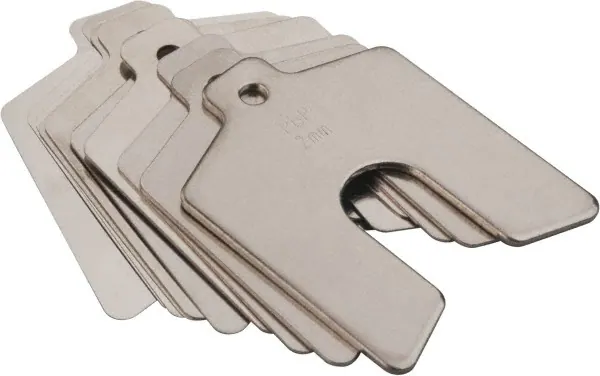
\includegraphics[scale=0.25]{Images/shims.png}
		\captionof{figure}{{\it Shims} of various thicknesses}
		\small\textsuperscript{Source: www.mscdirect.com/product/details/70475967}
		\label{fig:shims}
		
	\end{minipage}\hfill % these two lines must be close to each other
	\begin{minipage}{0.58\linewidth}
		
		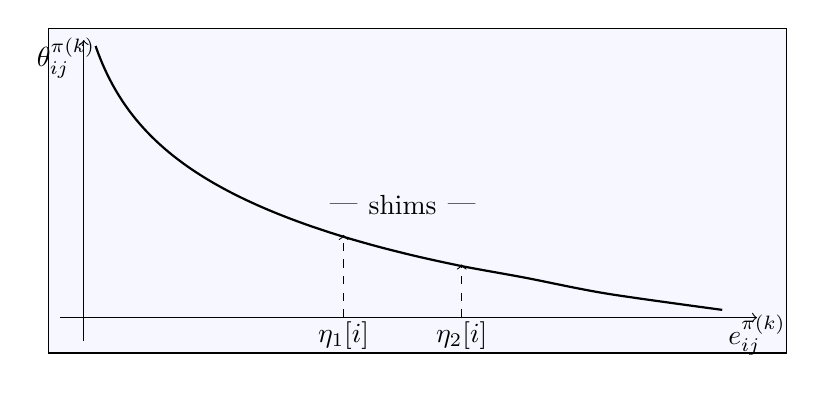
\begin{tikzpicture}[scale=0.75, samples=100]
			\filldraw[fill=blue!3!white, draw=black] (0, 0) rectangle (12.5, 5.5);
			\draw[->] (.2, .6) -- coordinate (x axis mid) (12, .6);
			\node at (5, 0.3) {$\eta_1[i]$};
			\node at (5, 2.5) {|};
			\node at (6, 2.5) {shims};
			\node at (7, 2.5) {|};
			\node at (7, 0.3) {$\eta_2[i]$};
			\node at (0.3, 5) {$\theta_{ij}^{\pi(k)}$};
			\draw[->] (.6, .2) -- coordinate (y axis mid) (0.6, 5.3);
			\node at (12, 0.3) {$e_{ij}^{\pi(k)}$};
			\draw[smooth, domain = 0.09:2, color=black, thick] plot (.3+1/\x,{4.2+log2(\x)});
			\draw[->, dashed] (5, 0.6)--(5, 2.0);
			\draw[->, dashed] (7, 0.6)--(7, 1.5);
		\end{tikzpicture}
		
		\captionof{figure}{$n_{\pi(k)}$\/ edges $e_{ij}^{\pi(k)}$\/ of $p_i$\/ sorted by $\theta_{ij}^{\pi(k)}$\/ in non-ascending order}
		\label{fig:whip}		
	\end{minipage}
\end{table}


Figure \ref{fig:whip} represents the $n_{\pi(k)}$\/ possible edges $e_{ij}^{\pi(k)}$\/ of $p_i$\/ sorted by $\theta_{ij}^{\pi(k)}$. \emph{Shims}\/ starts with a greedy solution, stopping at the edge with index in $\eta_1[i]$ close to the local optimum (first phase). Then, considering even the edge with the index $\eta_2[i]$, it elaborates different possible complements for this pallet and selects the best of these complements (second phase).

Although the second phase solves a knapsack problem, an algorithm for solving a Bin Packing Problem was used (the First Fit Decreasing - FFD), and the most profitable bin (Shims) was selected. This method was proved to be faster than a Dynamic Program solution for the Knapsack Problem.
		
	In this work, we included a new phase after the first: a minimization of the CG deviation. An integer programming procedure that helps improve the overall {\it mpShims} results.

$1^{st}$ - A Greedy phase to partially build pallets.

$2^{st}$ - Minimization of CG deviation.

$3^{st}$ - {\it Shims} set construction and best {\it Shims} selection

All executed in a multi-process execution, accessing concurrently, reading and writing, the list of items and the current value of the CG deviation.
As to the multi-process execution, we considered each pallet as a process.



\subsection{mpShims}


\begin{algorithm}[H]
	\caption{$mpShims$ main process}  \label{alg:mpShims}
	
	\begin{algorithmic}[1]
		
		\Procedure{$mpShims$}{${N_{\pi(k)}, \pi(k)}, limit, G$}
		
		\State Let $G(M,\ Q_{\pi(k)},\ E_{\pi(k)})$ \label{mpShims:g1} \Comment{the initial solution solution}
		
		\State $surplus \gets 1 + 3 \times (1 - limit)$
		
		\State $nodeTorque \gets 0$
		
		\State $ts \gets 2.0$ \Comment{torque surplus} \label{mpShims:ts}
		
		\State $lock \gets$ multi-processing lock  \label{mpShims:lock} \Comment{avoid race condition}
		
		\State $proc \gets \{p_1,p_2,..., p_m\}$  \Comment{each pallet has its own process}
		
		\For{$i \gets 1$ to $m$}
		\State $proc_i \gets Greedy(p_i,\ N_{\pi(k)},\ \pi(k),\ nodeTorque,\ G,\ limit,\ lock,\ ts )$   \label{mpShims:greedy}
		\State $proc_i.start$
		\EndFor
		
		\For{$i \gets 1$ to $m$}
		\State $proc_i.join$ \label{mpShims:join1}
		\EndFor
		
		\State $minCGdev(M,\ \pi(k),\ nodeTorque)$  \label{mpShims:minCGdev} \Comment{minimize the CG deviation.}
		
		\For{$i \gets 1$ to $m$}
		\State $proc_i \gets getBestShims(p_i,\ N_{\pi(k)},\ \pi(k),\ nodeTorque,\ G,\ surplus,\ lock,\ ts )$ \label{mpShims:getBestShims}
		\State $proc_i.start$
		\EndFor
		
		\For{$i \gets 1$ to $m$}
		\State $proc_i.join$ \label{mpShims:join2}

		\EndFor
		
		\Return $G(M,\ N_{\pi(k)} \cup Q_{\pi(k)},\ E_{\pi(k)})$ \label{mpShims:return}
		
		\EndProcedure
		
	\end{algorithmic}
\end{algorithm}

Line \ref{mpShims:g1} the initial solution comes with some consolidated on board, a bipartite graph between pallets and consolidated.

Line \ref{mpShims:ts} defines the torque surplus ($ts$). For the greedy phase, the solution may generate torque infeasible solutions with doubled torque ($2.0$), which will be repaired by the next phase, the minimization of the CG deviation.

Line \ref{mpShims:lock} creates a lock feature for shared data among processes to avoid race condition.

Line \ref{mpShims:greedy} calls the greedy method which updates $p_i$, $N_{\pi(k)}$, $nodeTorque$, and $G$.

Line \ref{mpShims:join1} wait for all $Greedy$ processes to finish.

Line \ref{mpShims:minCGdev} calls the $minCGdev$ integer programming method (Subsection \ref{subsection:second_phase}) which updates the $nodeTorque$ and $G$. $minCGdev$ minimizes the CG deviation. We raise the hypothesis that, in sequential mode, where one pallet is built at a time, torque constraints may be more restrictive than volume or weight constraints, which could stop the palletization process earlier, fostering a solution that may be not as good as it could be. So, we decided to balance cargo before the next {\it Shims} phase to allow more room for pallet fulfillment. This will be confirmed (or not) in Section \ref{sec6}.

Line \ref{mpShims:getBestShims} calls the $getBestShims$ method which updates $p_i$, $N_{\pi(k)}$, $nodeTorque$, and $G$.

Line \ref{mpShims:join2} wait for all $getBestShims$ processes to finish.

Line \ref{mpShims:return} returns a complete solution, a bipartite graph between pallets and consolidated or items.

\subsubsection{{\it Shims} first phase}


Algorithm \ref{alg:greedy} generates a greedy allocation of the items available in node $l_{\pi(k)}$, according to the non-ascending order of $\theta^{\pi(k)}_{ij}$, and considering the consolidated items already shipped ($E^Q_{\pi(k)}$). Edges are included in this allocation as long as they respect feasibility constraints. Furthermore, the volume of each pallet $p_i$\/ cannot exceed $p_i.v \times limit$, where $ 0 < limit \leq 1$\/ is a given parameter.

\begin{algorithm}[H]
	\caption{Mount a greedy solution until the volume limit for each pallet}  \label{alg:greedy}
	
	\begin{algorithmic}[1]
		
		\Procedure{$Greedy$}{${\pi(k)}, G, limit$}
		
		\State Let $G(V_{\pi(k)}, E^Q_{\pi(k)})$
		
		\State $\eta_1 \gets \{0\} \times m$ \label{greedy:eta}
		\State $volume \gets \{0\} \times m$
		
		\State $E^N_{\pi(k)} \gets \varnothing$ 			
		
		\For{$q \gets 1$ to $m$}
		\If{$(p_i, a_q^{\pi(k)}) \in E^Q_{\pi(k)}$} 
		\State $volume[q] \gets volume[q] + a_q^{\pi(k)}.v$ 
		\EndIf		
		\EndFor
		
		\For {each $e_{ij}^{\pi(k)}$ in non-ascending order of $\theta^{\pi(k)}_{ij}$}
		\If{($E^N_{\pi(k)} \cup \{e_{ij}^{\pi(k)}\}$ is feasible) {\bf and} ($volume[i] \leq p_i.v \times limit$)} 
		\State $E^N_{\pi(k)} \gets E^N_{\pi(k)} \cup \{e_{ij}^{\pi(k)}\}$ 
		\State $volume[i] \gets volume[i] + t_j^{\pi(k)}.v$
		\State $\eta_1[i] \gets \eta_1[i] + 1$ 	
		\EndIf
		\EndFor
		
		\Return $G(V_{\pi(k)}, E^N_{\pi(k)} \cup E^Q_{\pi(k)}),\ \eta_1$ \Comment{return the partial solution and the last item indexes array }
		
		\EndProcedure
		
	\end{algorithmic}
\end{algorithm}

In Algorithm \ref{alg:greedy}, line \ref{greedy:eta} defines an array with the same size as pallets array to save the set of last edges inserted in the greedy solution. The set $\eta_1$ is returned together with the greedy solution.



\subsubsection{{\it Shims} second phase: improvement on minimizing CG deviation}
\label{subsection:second_phase}

Between the greedy and the {\it Shims} selection phases we inserted, in this work, an integer programming method to minimize the CG deviation, as stated by the model that follows.

Let $\pi$ be a tour in the set of permutations of nodes.

Let $Q^{\pi(k)}  = \{ a^{\pi(k)}_1, a^{\pi(k)}_2, \ldots, a^{\pi(k)}_m \}$ be the set of consolidated items assembled on the set of $m$ pallets in node $\pi(k)$. There is a bi-univocal relation between pallets and consolidated.

Let $H^{\pi(k)}_{iq}$ be the set of decision variables that relates pallet $i$ to consolidated $q$ in node $\pi(k)$.

\begin{equation} \label{eq:distobjshims}
	\mbox{minimize}\ \Bigg |  \sum_{i=1}^{m} \sum_{q=1}^{m} H^{\pi(k)}_{iq} \times  (140 + a^{\pi(k)}_q.w) * p_i.d\ \Bigg | 
\end{equation}

\begin{equation} \label{eq:distconsshims}
	s.t.: \sum_{i=1}^{m} H^{\pi(k)}_{iq} = 1;\ q \in \{1,2,\ldots,m\}
\end{equation}

\begin{equation} \label{eq:distpalletsshims}
	s.t.: \sum_{q=1}^{m} H^{\pi(k)}_{iq}=1;\ i \in \{1,2,\ldots,m\}
\end{equation}

Equation \ref{eq:distobjshims} minimizes the aircraft absolute torque in node $\pi(k)$, where 140 is the weight of an empty pallet, $a^{\pi(k)}_q.w$ the weight of the consolidated, and $p_i.d$ the distance between the pallet centroid to the aircraft CG; Equation \ref{eq:distconsshims} states that each consolidated will be assigned to exactly one pallet; and Equation \ref{eq:distpalletsshims} states that each pallet will receive one consolidated.


\subsubsection{{\it Shims} third phase}

\begin{algorithm}[H]
	\caption{Mount shims of edges that fills each pallet gap and return the best shims}  \label{alg:getBestShims}
	\begin{algorithmic}[1]
		
		\Procedure{$getBestShims$}{$i,\ \eta_1,\ \eta_2,\ E,\ k,\ slack$}
		
		\State $volume \gets 0$	
		
		\State $b \gets 1$
		\State $shims[b] \gets \{\}$  \label{empty_shims}
		\State $Set \gets Set \cup \{shims[b]\}$ \label{empty_set}
		
		\For{$x \gets \eta_1[i]$ to $\eta_2[i]$} \label{edges_indexes}
		
		
		\State $NewShims \gets$ {\bf True} \label{new_shims}
		\State $e_{ij}^k \gets E[i][x]$
		
		\For{$shims \in Set$} \label{shims_set}
		
		\If { $e_{ij}^k \not\in (E^N_k \cup shims)$ {\bf and} $e_{ij}^k$ is feasible  {\bf and}  $(t_j^k.v + volume) \leq slack[i]$}
		
		
		\State $shims \gets shims \cup \{e_{ij}^k\}$
		\State $volume \gets volume + t_j^k.v$
		\State $NewShims \gets$ {\bf False} \label{new_shims_false}
		
		\State {\bf break}
		
		\EndIf
		
		\EndFor 
		
		\If{$NewShims$} \label{new_shims2}
		\State $volume \gets 0$
		\State $b \gets b + 1$
		\State $shims[b] \gets \{\}$
		\State $shims[b] \gets shims[b] \cup \{e_{ij}^k\}$
		\State $Set \gets Set \cup \{shims[b]\}$
		\EndIf
		
		\EndFor 
		
		\State $sh_w \gets shims$, where $shims \in Set$ and $\sum_{e_{ab}^k \in shims} t_b^k.w$ is maximum  \label{best_weight}		
		\State $sh_v \gets shims$, where $shims \in Set$ and $\sum_{e_{ab}^k \in shims} t_b^k.v$ is maximum \label{best_volume}
		\State $sh_{best} \gets shims$, where $shims \in \{sh_w, sh_v\}$ and $\sum_{e_{ab}^k \in x} t_b^k.s$ is maximum \label{best_score}
		
		\Return $sh_{best}$
		
		\EndProcedure
		
	\end{algorithmic}
\end{algorithm}

Algorithm \ref{alg:getBestShims} describes the procedure to get the top {\it Shims}, the best subset of edges to fill each pallet gap. This algorithm follows the logic of the {\it First-Fit Decreasing} method as described by \cite{JohnsonGarey1985}. Although it does not aim to minimize the number of bins, its mechanism helped build the set of {\it Shims} to allow the best to be chosen.

Line \ref{empty_shims} creates the first empty shims.
Line \ref{empty_set} produce the first set of shims from where the best shims will be chosen.

Line \ref{edges_indexes} iterate in the edges indexes range to find subsets of shims that fit into each pallet gap.

Initially, new shims creation is permitted (\ref{new_shims}), but it will only be created if the last edge could not be included in any shims from the set (\ref{new_shims2}). 

For each edge, iterate in all sets in a try to include it in any of the previous shims (\ref{shims_set}).
As the last edge was included, forbid a new shims creation (\ref{new_shims_false}).

Finally, select the best weight shims (\ref{best_weight}), the best volume shims (\ref{best_volume}), and the best score shims (\ref{best_score}) between these 2. The best score shims edges will be returned.



\section{Implementation and results}
\label{sec6}


As we are dealing with a new problem, which has been modeled by \cite{MesquitaSanches2023}, we use the same benchmarks of their work, which are based on the characteristics of real airlifts carried out by the {\em Brazilian Air Force}.
 
We test our methods with 126 different instances: six operational scenarios with 2 aircraft sizes and 3 to 7 nodes; and seven randomly generated item sets for three volume surpluses (1.2, 1.5, and 2.0 times aircraft volume capacities).


\subsection{Results obtained}

The final experiments are performed on a 64-bit, 16GiB, 3.6GHz, 8-core AMD® Fx-8320e processor, 2 threads per core, with {\it Linux Ubuntu 20} as the operational system and {\it Python 3.8.2} as the programming language.

A relevant problem with meta-heuristics is the parameter's adjustment to extract the best possible efficiency in the optimization. The bulk of the tools to fine-tune these parameters utilize a statistical backdrop that enables them to make accurate predictions regarding the differences in candidate configurations' performance. Inadequacies in the design of the statistical experiment may therefore lead to erroneous results from the statistical tests and, subsequently, cause the approach to produce inaccurate comparisons of candidate configurations. That is why all parameters were set using the $iRace$ package \citep{LopezIbanezManuel2016}. Supplying $iRace$ with a range for $volThreshold$ as [0.80 to 0.99], {\it iRace} yielded 0.92, by training on the uneven instances numbers. The values tested for 20\%, 50\%, and 100\% volume surpluses were very close, considering the confidence level offered by {\it iRace}.

For parallelization, we used the {\it Python Multi-processing} package, which implements {\it process-based parallelism} or {\it parallel shared memory algorithm}. According to \cite{multiprocessing}, {\it Multi-processing} is a package that supports spawning processes using an API similar to the {\it Python Threading} package.

According to \cite[p.271]{Breshears2009}, a {\it Process} is the operating system’s spawned and controlled entity that encapsulates an executing application. A process has two main jobs: the first is to hold the application's resources, and the second is to carry out the application's instructions. 

It is known that working concurrently opens up synchronization issues. But the {\it Multi-processing} package (mp) offers both local and remote concurrency, effectively side-stepping the global interpreter lock by using sub-processes instead of threads. Because of this, the {\it Multi-processing} module lets the programmer take full advantage of the fact that a machine has more than one processor, normally capable of 2 threads each.

By Amdahl's law, there is an optimal number of parallel executions for each problem in each environment. While working at IBM in 1967, Gene Amdahl developed the foundation for what became known as Amdahl's Law or Amdahl's Argument. Essentially, the law states that while a process can be decomposed into steps that may then be run in parallel, the time taken for the whole process will be significantly limited by the steps that remain serialized.

We ran Algorithm \ref{alg:main} in the 6 scenarios described in Table \ref{tab:scenarios}, considering 3 methods for node-by-node resolution: the {\it Gurobi} MIP solver, {\it Shims}, and {\it mpShims} (Algorithm \ref{alg:mpShims}).

In generating the items in each node, we consider 3 values for the parameter ${\it surplus}$. The results obtained for the function $f$, with the corresponding run time in seconds, are shown in Tables \ref{tab:results} (${\it surplus} = 1.2$, ${\it surplus} = 1.5$, and ${\it surplus} = 2.0$).

For each $method$, $scenario$ and $surplus$, 7 different instances were generated. Therefore, 126 tests (6 scenarios $\times$ 3 volumes $\times$ 7 instances) were performed for each method. 

The average tour values were presented for $f$ and, for the run time, the worst result obtained. To facilitate the comparison between the methods, we added a last column in these tables, where two values are indicated:
\begin{itemize}
	\item {\bf Normalized}: value between 0 and 1, which corresponds to the ratio between the sum of $f$\/ values obtained by the method in all scenarios and the sum of the best values obtained among all methods in all scenarios. The higher the value of {\bf Normalized}, the closer the method approached the best solutions found.
	\item {\bf Speedup}: ratio of the sums of the worst runtimes of all scenarios and the sum of the method runtimes in all scenarios. The method with the highest {\bf Speed-up}\/ is the fastest.
\end{itemize}

In each $scenario$, we indicate in bold the best value of $f$\/ found. In each table, we also indicate in bold the best {\bf Normalized}\/ and {\bf Speed-up}\/ values.

\vspace{2.0mm}

\begin{table}[H]
	\centering
	\caption{Volume surpluses, methods and scenarios results}  \label{tab:results}
	\footnotesize
	%\scriptsize
	\begin{tabular}{crcccccccc}
		\toprule
		{\bf Volume}     &  {\bf Resolution}   &                              &\multicolumn{6}{c}{\bf Scenarios}                                                   &{\bf Normalized}\\
		\cmidrule{4-9}		
		{\it surplus}    & {\it method}        & {\bf Results}                &{\bf 1}    &{\bf 2}    &{\bf 3}    &{\bf 4}    &{\bf 5}    &{\bf 6}    &{\bf Speedup} \\
		\toprule
		
		%\specialcell{$Volume$\\$surplus$}
		
		\multirow{6}{*}{$1.2$}&\specialcell{$Relaxed$\\$Gurobi$}& $f$         &{\it 12.23}&{\it 8.67} &{\it 12.67}&{\it 15.36}&{\it 16.29}&{\it 16.20}&  \specialcell{{\bf 1.00}\\-} \\%  8142
		
		\cmidrule{2-10}		                       
		&\multirow{2}{*}{ $Shims$}                       & $f$                &     10.34 &     8.50  &     12.42 &     15.06 &     15.97 &     15.88 &  0.96 \\% 7817
		&                                                & {\it run time (s)} &     < 1   &     3     &     5     &     20    &     58    &     352   &  1.0 \\% 439			
		\cmidrule{2-10}		                       
		&\multirow{2}{*}{ $mpShims$}                     & $f$                &   12.96   &   7.53    &  12.28    &   13.20   &  13.71    &   13.44   &  0.90\\% 7278
		&                                                & {\it run time (s)} &     < 1   &     2     &     2     &     8    &     22    &     120   &  {\bf 2.8}\\%
		
		\midrule		
		
		\multirow{6}{*}{$1.5$}&\specialcell{$Relaxed$\\$Gurobi$}& $f$         &{\it 17.01}&{\it 12.45}&{\it 18.02}&{\it 22.03}&{\it 23.09}&{\it 22.35}&  \specialcell{{\bf 1.00}\\-} \\%11495  

        \cmidrule{2-10}		                       
        &\multirow{2}{*}{ $Shims$}                       & $f$                &     14.68 &     12.21 &     17.67 &  21.01    &  22.64    &   21.91   &  0.96  \\%  11012
        &                                                & {\it run time (s)} &     < 1   &     2     &     3     &     12    &     33    &   209     &  1.0 \\% 260

        \cmidrule{2-10}		                       
        &\multirow{2}{*}{ $mpShims$}                     & $f$                &    16.12  &     11.81 &     17.48 &  17.66    &   19.81   &  17.61    &  0.87 \\% 9966
        &                                                & {\it run time (s)} &     < 1   &     1     &     2     &     7     &   20      &  120      &  {\bf 1.7}\\% 151

		\midrule
		\multirow{6}{*}{$2.0$}&\specialcell{$Relaxed$\\$Gurobi$}& $f$         &{\it 24.56}&{\it 17.47}&{\it 25.19}&{\it 27.94}&{\it 29.90}&{\it 27.60 }&  \specialcell{{\bf 1.00}\\-} \\%15266  
		
		\cmidrule{2-10}		                       
		&\multirow{2}{*}{ $Shims$}                       & $f$                &    21.31  &  17.35    &   24.24   &   27.39    &  29.31     &  27.06     &   0.96  \\%  14666
		&                                                & {\it run time (s)} &     < 1   &     2     &     4     &     14     &     35     &   220     &  1.0 \\% 260
		
		\cmidrule{2-10}		                       
		&\multirow{2}{*}{ $mpShims$}                     & $f$                &    24.33  &   17.26   &   24.70   &  24.81     &   27.71    &  24.93        &  0.94  \\% 14374
		&                                                & {\it run time (s)} &     < 1   &     2     &     3     &     9      &   26       &  151      &  {\bf 1.7}\\% 151

		\bottomrule	
		
	\end{tabular}
	%\textsuperscript{asdf sd .}	
	\normalsize
\end{table}

The upper bound is the objective function value of a linear programming relaxation of the problem, demonstrating that no integer viable solution can have an objective value greater (in maximization) than this.

We solved all scenarios and instances with {\it Gurobi} in a relaxed linear model, {\it Relaxed Gurobi}. This is good for the reader to have an idea of the real performance differences between serial and parallel {\it Shims}.

{\it Shims} had a quality performance very close to the {\it Relaxed Gurobi} upper bound solution, and, as to the {\bf Speedup}, on average, {\it mpShims} was 2 times faster than {\it Shims}. Theoretically, it could be more, but due to the burden of sharing, for reading and writing, the CG deviation and the list of items among the processes (pallets), the {\it race condition} management limited {\it mpShims} performance.

{\it When threads or processes attempt to simultaneously access a shared resource, and the accesses can result in an error, we often say the program has a race condition, because the threads or processes are in a "race" to carry out an operation.} \cite[p. 53]{Pacheco:2020}.

We confirmed the hypothesis raised in line \ref{mpShims:minCGdev} of Algorithm \ref{alg:mpShims} that, in sequential mode, where one pallet is built at a time, torque constraints could be more restrictive than volume or weight constraints, which could stop the palletization process earlier, fostering a solution that may be not as good as it could be. This integer programming procedure inclusion really improved all {\it Shims} results.

After this inclusion {\it Shims} results surpassed that of {\it mpShims}. In multi-processing mode ({\it mpShims}) this inclusion (line \ref{mpShims:minCGdev}) made a negligible difference.

\subsection{Another possible improvement}
\label{improvement}

\cite{LurkinSchyns2015} considered an aircraft with two doors, and the minimization of loading and unloading costs at the intermediate node was modeled through a container sequencing problem. But, as both aircrafts dealt with in this work have only the ramp door, we tried to minimize the distance of travel of pallets inside the cargo bay, favoring unloading in the next node, by a post optimization of pallets positions to favor this distance minimization.

So, to confirm or not Hypothesis (3), that the distances to move pallets on unloading in the next node could be minimized to benefit unloading costs. We modeled this improvement as follows.

Let $maxD$ be the distance from the last ramp pallet to the center of gravity.

Let $Q^{\pi(k)}  = \{ a^{\pi(k)}_1, a^{\pi(k)}_2, \ldots, a^{\pi(k)}_m \}$ be the set of consolidated items assembled on the set of $m$ pallets in node $\pi(k)$.

Let $Z^{\pi(k)}_{iq}$ be the set of binary decision variables that relates pallet $i$ to consolidated $q$ in node $\pi(k)$.

\begin{equation} \label{eq:distobj}
	\mbox{minimize} \sum_{i=1}^{m} \sum_{q=1}^{m} Z^{\pi(k)}_{iq} \times ( maxD - p_i.d) ,\ \mbox{{\bf if}}\ a^{\pi(k)}_q.to = \pi(k+1) \}
\end{equation}

\begin{equation} \label{eq:distcons}
	s.t.: \sum_{i=1}^{m} Z^{\pi(k)}_{iq} = 1;\ q \in \{1,2,\ldots,m\}
\end{equation}

\begin{equation} \label{eq:distpallets}
	s.t.: \sum_{q=1}^{m} Z^{\pi(k)}_{iq}=1;\ i \in \{1,2,\ldots,m\}
\end{equation}

\begin{equation} \label{eq:distpalletw}
	p_i.w = 140 + a^{\pi(k)}_q.w ;\ i \in \{1,2,\ldots,m\};\ q \in \{1,2,\ldots,m\}
\end{equation}

\begin{equation} \label{eq:disttorque}
	s.t.:\ | \sum\ p_i.d * p_i.w\ | \leq maxW \times limit^{CG}_{long} ;\ i \in \{1,2,\ldots,m\}
\end{equation}

Equation \ref{eq:distobj} minimizes the sum of distances of the consolidated in node $\pi(k)$ destined to the next node $\pi(k+1)$; Equation \ref{eq:distcons} states that each consolidated will be assigned to exactly one pallet; Equation \ref{eq:distpallets} states that each pallet will receive one consolidated; Equation \ref{eq:distpalletw} calculates the total weight of each pallet; and Equation \ref{eq:disttorque} guarantees that the torque limit will not be exceeded. 

As the number of pallets was small (7 or 18) for an integer program solver, the increased time was negligible (less than 1s).

There was some expectation on this post-improvement method as it could have minimized the distances of travel of the pallets through the ramp door, but unfortunately, after running all scenarios and problem instances, there was no improvement in minimizing these distances.

This proves that the solutions provided by {\it Shims} and {\it mpShims} are tight enough to hinder this intended improvement.

\subsection{Discussion summary}

In this work, we raised three hypotheses for improvements to the work of \cite{MesquitaSanches2023}:

(1) Computer parallelism could improve {\it Shims}'s performance: {\it mpShims} was twice as faster as {\it Shims}. This hypothesis was confirmed.

(2) The {\it Shims}' results may have been inferior in that of \cite{MesquitaSanches2023}; it could be that a sequential approach to pallet building may have lead to a premature stop due to the torque constraints. This hypothesis was confirmed as the results were improved by 5\% on average with the inclusion of a CG balancing integer programming procedure.

(3) The distances to move pallets on unloading in the next node could be minimized to benefit unloading costs. This hypothesis was not confirmed. We implemented an integer programming procedure to minimize these distances, but the results proved that any change in {\it Shims} or {\it mpShims} outcomes could turn the solutions unfeasible due to the CG balance constraints.

A new question is raised about whether it is worth using parallelism as, although {\it mpShims} was twice as fast as {\it Shims}, the results of {\it Shims} were still better than those of {\it mpShims}. May this question be solved through the real-world application of these methods.

\section{Conclusions}
\label{sec7}

In this work we dealt with a hard problem, named {\it Air Cargo Load Planning with Routing, Pickup, and Delivery Problem} considering standardized pallets in fixed positions, obeying the center of gravity constraints, delivering each item to its destination, and minimizing fuel consumption costs.

We converted \cite{MesquitaSanches2023} {\it Shims} into a process-based parallel computing heuristic, which we called {\it Multiprocessing Shims} or {\it mpShims}, that quickly finds good solutions for a wide range of problem sizes, our first contribution.

We also carried out 126 experiments with each method on synthetic data based on real data from the {\it Brazilian Air Force} transportation history.

Other important contributions are that we checked three hypotheses: Computer parallelism improved {\it Shims} performance; the intermediate integer programming procedure added to {\it Shims} algorithm enhanced it's results; but the integer programming procedure to minimize pallets' travel in the cargo bay did not improve the results. 

And another important contribution is that we employed the {\it iRace} package \citep{LopezIbanezManuel2016} to fine tune the {\it mpShims} volume threshold parameter, guaranteeing the best possible performance for the instances under training and testing.

\section*{Acknowledgments}

This research was partially supported by \textit{São Paulo Research Foundation} (FAPESP, grant 2016/01860-1).

%\bibliographystyle{elsarticle-num} % descomentar antes de submeter
\bibliographystyle{elsarticle-harv} % comentar antes de submeter

%\section*{References}

\bibliography{references}

\end{document}
